% \authornote{
%    \addORCIDlink{Ward B. Eiling}{0009-0007-8114-9497}
%   Correspondence concerning this article should be addressed to Daniel A. Weiss, Department of Educational Psychology, Counseling and
%   Special Education, A University Somewhere, 123 Main St., Oneonta, NY
%   13820.  E-mail: daniel.weiss.led@gmail.com}

\begin{document}

\maketitle

% Start the manuscript

% \subsection{Paragraph 1: Set the stage}

Across a wide range of disciplines, researchers analyze clustered longitudinal data to investigate prospective causal relationships between variables. When analyzing such data, psychological researchers commonly use the multilevel linear modeling (MLM) framework \parencite[]{bauer_fitting_2011}. A fundamental concern within the MLM literature is that the relationship between a predictor and an outcome may differ across levels of analysis \parencite[e.g.,][]{enders_centering_2007, kreft_effect_1995, raudenbush_hierarchical_2002}. In the context of longitudinal data, this implies that relationships across time captured at the within-person level of a model may differ from stable, between-person relationships as captured at the between-person level of a model. This discrepancy, known as the \textit{contextual effect}, is particularly important because failing to account for it results in an ``uninterpretable blend'' of within- and between-cluster relationships \parencite[139]{raudenbush_hierarchical_2002}. This blending obscures the within-person effect, which is typically the primary target of inference or causal interpretation.

% \subsection{Paragraph 2: Build up the tension}

The MLM literature offers several methods to disentangle within-person from between-person effects \parencite[]{curran_disaggregation_2011}. These include (a) person-mean centering of predictor variables and (b) entering uncentered predictors alongside cluster means as predictor of the random intercept \parencite[]{kreft_effect_1995, raudenbush_hierarchical_2002, bell_explaining_2015}. However, this body of work has primarily focused on continuous predictors, with limited guidance on how to disentangle effects when dealing with binary predictors. As a result, applied researchers may default to intuition or omit centering altogether when analyzing categorical predictors \parencite[]{yaremych_centering_2023}. This issue is exacerbated in generalized linear multilevel modeling (GLMM)\footnote{We refer to GLMM as the general modeling framework that includes MLMs for continuous outcomes and multilevel logistic models for binary outcomes.} with binary \textit{outcomes}, where the non-linearity between predictor and outcome further complicates interpretation \parencite[]{austin_intermediate_2017, bolger_intensive_2013}. This gap in methodological guidance is concerning since binary variables are ubiquitous within the social sciences and researchers may be left unaware of how to specify their models correctly. 

% \subsection{Paragraph 3: Build up the tension even more}

An established alternative for analyzing clustered data is the Generalized Estimating Equations (GEE) framework. It was originally developed in the biostatistics literature to accommodate longitudinal designs with non-normal outcomes, such as binary variables \parencite[]{liang_longitudinal_1986}. In biomedical studies, GEE is widely used—and often favored over GLMMs—for modeling binary outcomes \parencite[cf.][]{diggle_analysis_2002}. An important strength of GEE is its reliance on fewer unverfiable assumptions compared to GLMM \parencite[]{mcneish_unnecessary_2017, hubbard_gee_2010}. As GEE gains traction in psychology, researchers familiar with MLM may question how GEE compares to GLMMs and specifically whether the debate about separating within- from between-person effects using a method from MLM also applies when a GEE approach is taken. While some prior work has addressed how to handle binary predictors in MLMs \parencite{yaremych_centering_2023, enders_centering_2007, raudenbush_hierarchical_2002} or binary outcomes in GLMMs \parencite{bolger_intensive_2013, schunck_within-_2017}, and others have compared modeling frameworks across disciplines \parencite{mcneish_unnecessary_2017, ballinger_using_2004, yan_comparing_2013, muth_alternative_2016, neuhaus_comparison_1991}, no study to date has examined how different disaggregation methods perform across modeling frameworks and variable types. 

% \subsection{Paragraph 4: Aim of the Current Study (potential resolve?) and outline }

This paper seeks to address this gap by offering a systematic comparison of modeling approaches not yet synthesized in the current literature. Specifically, the goal of this paper is twofold. First, we aim to clarify how we should think about within and between effects with a binary predictors and/or outcomes. Second, we study the degree to which we can correctly estimate these effects with GLMM and GEE implementations. This article is structured as follows. We outline four data-generating models to conceptualize within-person and contextual effects across different measurement scales, supported by a running example. Next, we discuss modeling frameworks and methods for including predictors. We then present a simulation study in which we assess estimation performance across variations in (a) modeling approach (GLMM vs. GEE), (b) predictor inclusion strategies, (c) measurement levels (binary vs. continuous), and (d) sample size at both cluster and within-cluster levels. We evaluate when common modeling choices may lead to biased or misleading interpretations and provide practical guidance for applied researchers working with clustered binary data. We conclude with a summary of key findings, limitations, and directions for future research. 

\section{Data Generating Models}

In this section we describe the four data generating models (DGMs) that are used to clarify the within/between/contextual effects in the context of binary predictors and/or outcomes. These models form the basis of the simulation study. The DGMs differ in the measurement level of the predictor $X$ and the outcome $Y$ and are visualized in Figure~\ref{fig:path}. In all four DGMs we have a single time-varying predictor $X$, which is characterized by both stable differences at the between-level and variation within a person over time. Similarly, $Y$ is also a time-varying variable exhibiting both between-person stability and within-person fluctuations. $Y$ is affected by $X$ at two levels. At the within-level, moment specific deviations in \( X \) from an individual's stable mean influence their concurrent $Y$. At the between-level, stable differences in $Y$ are in part determined by stable differences in $X$.

To illustrate these DGMs, we use a running example grounded in prior empirical work on the effect of mindfulness (\(X_{it}\)) on anger (\(Y_{it}\)), where $X$ and $Y$ vary over individuals $i$ and timepoints $t$. Numerous studies have shown that, across individuals, those with higher overall mindfulness report lower overall levels of aggressiveness \parencite[]{brown_benefits_2003, borders_could_2010, kashdan_what_2016, baer_relationships_2011, eisenlohr-moul_both_2016}. Mindfulness also shows substantial within-person variability over time \parencite[]{brown_benefits_2003, kiken_state_2015}, and evidence suggests that on days when individuals report higher-than-usual mindfulness, they also report lower levels of state anger \parencite[]{eisenlohr-moul_both_2016}. Both within- and between-person associations are typically negative, though effect sizes depend on the specific operationalization \parencite{eisenlohr-moul_both_2016}. Nevertheless, between-person associations tend to be larger, consistent with trait mindfulness being a more stable and robust predictor of anger-related outcomes than day-to-day fluctuations.

\begin{center}
    \captionof{figure}{Path diagrams of Generative Models with Within-Person ($\beta_1$) and Contextual Effect ($\gamma_{01}$)}
    % Top row
    \begin{minipage}[t]{.49\linewidth}
        \centering
        \begin{subfigure}[b]{\linewidth}
            \centering
            
\includegraphics[height=6.5cm]{Figures/pathdiagrams-cropped-contxy.drawio.pdf}
            \caption{Continuous X and Y}\label{fig:path-contxy}
        \end{subfigure}
    \end{minipage}
    \hfill
    \begin{minipage}[t]{.49\linewidth}
        \centering
        \begin{subfigure}[b]{\linewidth}
            \centering
            
\includegraphics[height=6.5cm]{Figures/pathdiagrams-cropped-binxconty.drawio.pdf}
            \caption{Binary X and Continuous Y}\label{fig:path-binxconty}
        \end{subfigure}
    \end{minipage}

    % \vskip 1em

    % Bottom row
    \begin{minipage}[t]{.49\linewidth}
        \centering
        \begin{subfigure}[b]{\linewidth}
            \centering
            
\includegraphics[height=7.5cm]{Figures/pathdiagrams-cropped-contxbiny.drawio.pdf}
            \caption{Continuous X and Binary Y}\label{fig:path-contxbiny}
        \end{subfigure}
    \end{minipage}
    \hfill
    \begin{minipage}[t]{.49\linewidth}
        \centering
        \begin{subfigure}[b]{\linewidth}
            \centering
            
\includegraphics[height=7.5cm]{Figures/pathdiagrams-cropped-binxy.drawio.pdf}
            \caption{Binary X and Y}\label{fig:path-binxy}
        \end{subfigure}
    \end{minipage}
    \vspace{-0.5cm}
    \label{fig:path}
    \begin{flushleft}
    \begin{figurenote}
    Path diagrams of the four data-generating models, varying by predictor type $X$ (columns) and outcome type $Y$ (rows), each either continuous or binary. In all models, the outcome is regressed on the predictor, and the person-level predictor mean $\mu_X$ predicts the outcome intercept $\beta_0$, yielding a within-person slope $\beta_1$ and a contextual effect $\gamma_{01}$. Circles represent latent variables, squares observed variables. Solid arrows denote linear relations; dotted arrows indicate logit transformations (\texttt{plogis} in \texttt{R}); dashed arrows indicate Bernoulli sampling with probability $\pi$ (\texttt{rbinom} in \texttt{R}).
    
    % Path diagrams of four data generating models that vary in predictor type $X$ (column wise) and outcome type $Y$ (row wise), both of which are either continuous or binary. Models are based regressing the outcome variable on the predictor, while using the latent mean per person on the predictor $\mu_X$ to predict the intercept $\beta_{0}$ of the outcome. This results in the within-person slope $\beta_1$ and the contextual effect $\gamma_{01}$. Circles denote latent variables, squares denote observed variables, and arrows represent relationships. Solid arrows indicate linear associations, dotted arrows represent logit transformations (\texttt{plogis} in \texttt{R}), and dashed arrows indicate Bernoulli sampling with probability $\pi$ (\texttt{rbinom} in \texttt{R}).
    % Circles represent latent variables, squares represent observed variables, and arrows indicate relationships. Solid arrows denote linear associations, with a coefficient of 1 indicating a one-to-one relationship. Dotted arrows represent logit transformations (\texttt{plogis} in \texttt{R}), and dashed arrows represent Bernoulli sampling based on the probability $\pi$ (\texttt{rbinom} in \texttt{R}).
    \end{figurenote}
    \end{flushleft}
\end{center}

% \begin{center}
%     \captionof{figure}{Path diagrams of Generative Models with Within-Person ($\beta_1$) and Contextual Effect ($\gamma_{01}$)}
%     % Top row
%     \begin{minipage}[t]{.49\linewidth}
%         \centering
%         \begin{subfigure}[b]{\linewidth}
%             \centering
%             
\includegraphics[width=\linewidth, height=8cm, keepaspectratio]{Figures/pathdiagrams-contxy.drawio.pdf}
%             \caption{Continuous X and Y}\label{fig:path-contxy}
%         \end{subfigure}
%     \end{minipage}
%     \hfill
%     \begin{minipage}[t]{.49\linewidth}
%         \centering
%         \begin{subfigure}[b]{\linewidth}
%             \centering
%             
\includegraphics[width=\linewidth, height=8cm, keepaspectratio]{Figures/pathdiagrams-contxbiny.drawio.pdf}
%             \caption{Continuous X and Binary Y}\label{fig:path-contxbiny}
%         \end{subfigure}
%     \end{minipage}

%     % \vskip 1em

%     % Bottom row
%     \begin{minipage}[t]{.49\linewidth}
%         \centering
%         \begin{subfigure}[b]{\linewidth}
%             \centering
%             
\includegraphics[width=\linewidth, height=8cm, keepaspectratio]{Figures/pathdiagrams-binxconty.drawio.pdf}
%             \caption{Binary X and Continuous Y}\label{fig:path-binxconty}
%         \end{subfigure}
%     \end{minipage}
%     \hfill
%     \begin{minipage}[t]{.49\linewidth}
%         \centering
%         \begin{subfigure}[b]{\linewidth}
%             \centering
%             
\includegraphics[width=\linewidth, height=8cm, keepaspectratio]{Figures/pathdiagrams-binxy.drawio.pdf}
%             \caption{Binary X and Y}\label{fig:path-binxy}
%         \end{subfigure}
%     \end{minipage}
%     \vspace{-1cm}
%     \label{fig:path}
%     \begin{flushleft}
%     \begin{figurenote}
%     Circles represent latent variables, squares represent observed variables, and arrows indicate relationships. Solid arrows denote linear associations, with a coefficient of 1 indicating a one-to-one relationship. Dotted arrows represent logit transformations (\texttt{plogis} in \texttt{R}), and dashed arrows represent Bernoulli sampling based on the probability $\pi$ (\texttt{rbinom} in \texttt{R}).
%     \end{figurenote}
%     \end{flushleft}
% \end{center}

% \begin{center}
% \captionof{figure}{Path diagrams of Generative Models with Within-Person ($\beta_\text{w}$) and Contextual Effect ($\gamma_{01}$)}

% \begin{minipage}[t]{.49\linewidth}
%     \centering
%     \begin{subfigure}[b]{\linewidth}
%         \centering
%         
\includegraphics[width=\linewidth, height=8cm, keepaspectratio]{Figures/pathdiagrams-contxy.drawio.pdf}
%         \caption{Continuous X and Y}\label{fig:path-contxy}
%     \end{subfigure}
%     \vspace{1em}
%     \begin{subfigure}[b]{\linewidth}
%         \centering
%         
\includegraphics[width=\linewidth, height=8cm, keepaspectratio]{Figures/pathdiagrams-binxconty.drawio.pdf}
%         \caption{Binary X and Continuous Y}\label{fig:path-binxconty}
%     \end{subfigure}
% \end{minipage}
% \hfill
% \begin{minipage}[t]{.49\linewidth}
%     \centering
%     \begin{subfigure}[b]{\linewidth}
%         \centering
%         
\includegraphics[width=\linewidth, height=8cm, keepaspectratio]{Figures/pathdiagrams-contxbiny.drawio.pdf}
%         \caption{Continuous X and Binary Y}\label{fig:path-contxbiny}
%     \end{subfigure}
%     \vspace{1em}
%     \begin{subfigure}[b]{\linewidth}
%         \centering
%         
\includegraphics[width=\linewidth, height=8cm, keepaspectratio]{Figures/pathdiagrams-binxy.drawio.pdf}
%         \caption{Binary X and Y}\label{fig:path-binxy}
%     \end{subfigure}
% \end{minipage}

% \vspace{-0.5cm}
% \label{fig:path}

% \begin{flushleft}
% \begin{figurenote}
% Circles represent latent variables, squares represent observed variables, and arrows indicate relationships. Solid arrows denote linear associations, with a coefficient of 1 indicating a one-to-one relationship. Dotted arrows represent logit transformations (\texttt{plogis} in \texttt{R}), and dashed arrows represent Bernoulli sampling based on the probability $\pi$ (\texttt{rbinom} in \texttt{R}).
% \end{figurenote}
% \end{flushleft}
% \end{center}


\subsection{DGM 1: Continuous Predictor and Outcome}

To illustrate the DGM for a continuous predictor and outcome, we consider the case of how mindfulness relates to daily experiences of anger (see Figure~\ref{fig:path-contxy}). Each individual possesses a stable level of trait mindfulness, denoted as a person-specific latent mean \( \mu_{X,i} \). This latent trait is assumed to vary across individuals according to a normal distribution $\mu_{X,i} \sim \mathcal{N}(0, \sigma^2_{X,\text{b}})$, where \( \sigma^2_{X,\text{b}} \) reflects the between-person variance in mindfulness. The observed $X$ for individual \( i \) at occasion \( t \), denoted \( X_{it} \), is a combination of an individual's stable trait level and a momentary deviation:
\begin{align}
    \label{eqn:relationwithinmundlak}
    X_{it} &= \mu_{X,i} + X_{w,it}
\end{align}
Here, \( X_{w,it} \) represents within-person variability in mindfulness, capturing occasion specific fluctuations around the person’s trait level. These deviations vary over time according to a normal distribution \( X_{w,it} \sim \mathcal{N}(0, \sigma^2_{X,\text{w}}) \), where \( \sigma^2_{X,\text{w}} \) reflects within-person variance in mindfulness. Daily anger (\( Y_{it} \)) is a function of both levels of mindfulness. At the within-person level, we specify:
\begin{equation}
    \label{eqn:yit-generationmlm}
    Y_{it} = \beta_{0i} + \beta_{1} X_{it} + e_{it},
\end{equation}
where \( \beta_{0i} \) is an individual-specific intercept capturing baseline anger, \( \beta_1 \) is the fixed \textit{within-person effect} of mindfulness on anger, and \( e_{it} \sim \mathcal{N}(0, \sigma^2_e) \) is a person- and time-specific residual, which is normally distributed with variance $\sigma^2_e$. To introduce between-person effects, the individual-specific intercept \( \beta_{0i} \) is a function of the person’s average mindfulness:
\begin{equation}
    \label{eqn:beta0-generationcontxy}
    \beta_{0i} = \gamma_{00} + \gamma_{01} \mu_{X,i} + u_{0i},
\end{equation}
where \( \gamma_{00} \) is the grand mean of anger and \( \gamma_{01} \) is the contextual effect of trait mindfulness on anger. The person-specific residual \( u_{0i} \sim \mathcal{N}(0, \sigma^2_u) \) is normally distributed with variance \( \sigma^2_u \) and represents heterogeneity in baseline anger not explained by mindfulness. Substituting the between-person model into the within-person equation yields the full generative model:
\begin{equation}
    Y_{it} = \gamma_{00} + \gamma_{01} \mu_{X,i} + u_{0i} + \beta_1 X_{it} + e_{it}.
\end{equation}
In this DGM, there are two ways in which minfulness ($X$) influences anger ($Y$). The coefficient \( \beta_1 \) captures the within-person effect $\beta_\text{w}$, which is the extent to which anger changes when an individual is more or less mindful than usual. The \textit{contextual effect} \( \gamma_{01} \) captures the degree to which the between-person effect---the association between a person's typical mindfulness level (\( \mu_{X,i} \)) and stable anger level---differs from the within-person effect. The implied between-person effect is then given by $\beta_\text{b} = \gamma_{01} + \beta_1$ \parencite{mundlak_pooling_1978}.\footnote{This equivalence does not hold in the presence of \textit{random slopes} \parencite[cf.][]{snijders_multilevel_2011}.}  A positive \( \gamma_{01} \) implies that individuals who are more mindful on average experience more anger than would be expected based only on the within-person relationship. A negative \( \gamma_{01} \) implies that individuals who are more mindful on average experience less anger than would be expected based solely on the within-person relationship—suggesting a trait-level benefit of mindfulness. 

Empirical studies found that between-person effects may be larger in magnitude than within-person effects $\beta_\text{b} > \beta_\text{w}$. As both effects are negative, this implies the presence of a \textit{negative} contextual effect. To reflect this, we might specify the following parameter values $
\gamma_{00} = 4.5,\quad \gamma_{01} = -0.5,\quad \beta_1 = -0.4$ so that $\beta_\text{b} = -0.6 - 0.4 = -0.9$. As visualized in Figure~\ref{fig:withinbetween-contxy}, these parameters yield a stronger negative association at the between-person level than at the within-person level. We can observe that the within-person effect is identical for the two individuals, with the difference pertaining only to the random intercept $\beta_{0i}$: the person with the orange line has datapoints clustered around a greater trait-level of mindfulness ($\mu_{X,i} = 4$) than the person with the red line ($\mu_{X,i} = 2$). Due to the negative between-person effect of $X$ on $Y$, it follows that the person with the orange line also has lower overall anger levels.

\newpage
\begin{center}
    \captionof{figure}{Illustration of Within- and Between-Person Effects in Generative Models with $\beta_1 = -0.4$}
    % Top row
    \begin{minipage}[t]{.45\linewidth}
        \centering
        \begin{subfigure}[b]{\linewidth}
            \centering
            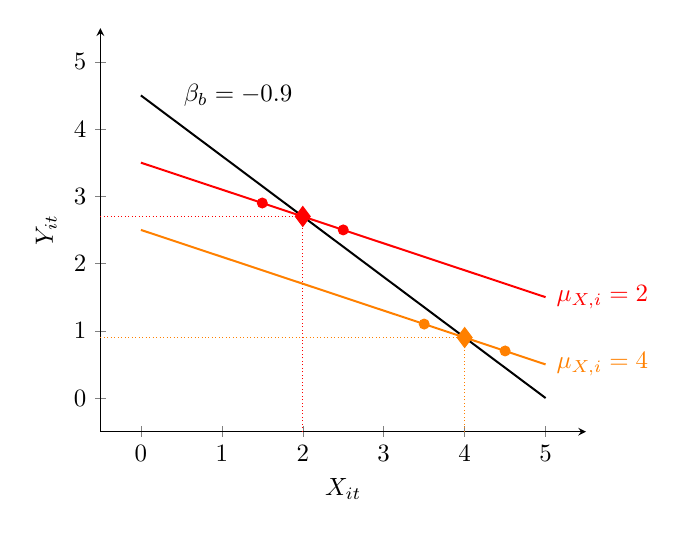
\begin{tikzpicture}[scale=0.9]
                \begin{axis}[
                    axis x line=left, 
                    axis y line=left, 
                    xlabel={$X_{it}$}, ylabel={$Y_{it}$},
                    xmin=0, xmax=5, ymin=0, ymax=5,
                    xtick={0,1,2,3,4,5},
                    ytick={0,1,2,3,4,5},
                    enlargelimits=true,
                    clip=false,
                    xshift=-15mm
                ]
            
                \pgfmathsetmacro{\gammaZero}{4.5}
                \pgfmathsetmacro{\gammaOne}{-0.5}
                \pgfmathsetmacro{\betaOne}{-0.4}
                \pgfmathsetmacro{\betaB}{-0.9}  % gamma01 + beta1
            
                % === Within-person: mu_X = 2 ===
                \addplot[domain=0:5, thick, red] {\gammaZero + \gammaOne*2 + \betaOne*x};
                \addplot[only marks, red] coordinates {
                    (1.5, {4.5 - 0.5*2 - 0.4*1.5})
                    % (2.0, {4.5 - 0.5*2 - 0.4*2.0})
                    (2.5, {4.5 - 0.5*2 - 0.4*2.5})
                };
                \addplot[only marks, mark=diamond*, mark size=4pt, red] coordinates {
                    (2.0, {4.5 - 0.5*2 - 0.4*2.0})
                };
                \addplot[densely dotted, thin, red] coordinates {
                    (2.0, -0.5)
                    (2.0, {4.5 - 0.5*2 - 0.4*2.0})
                };
                \addplot[densely dotted, thin, red] coordinates {
                    (-0.5, {4.5 - 0.5*2 - 0.4*2.0})
                    (2.0, {4.5 - 0.5*2 - 0.4*2.0})
                };
            
                % === Within-person: mu_X = 4 ===
                \addplot[domain=0:5, thick, orange] {\gammaZero + \gammaOne*4 + \betaOne*x};
                \addplot[only marks, orange] coordinates {
                    (3.5, {4.5 - 0.5*4 - 0.4*3.5})
                    % (4.0, {4.5 - 0.5*4 - 0.4*4.0})
                    (4.5, {4.5 - 0.5*4 - 0.4*4.5})
                };
                \addplot[only marks, mark=diamond*, mark size=4pt, orange] coordinates {
                    (4.0, {4.5 - 0.5*4 - 0.4*4.0})
                };
                \addplot[densely dotted, thin, orange] coordinates {
                    (4.0, -0.5)
                    (4.0, {4.5 - 0.5*4 - 0.4*4.0})
                };
                \addplot[densely dotted, thin, orange] coordinates {
                    (-0.5, {4.5 - 0.5*4 - 0.4*4})
                    (4.0, {4.5 - 0.5*4 - 0.4*4.0})
                };
            
                % === Between-person regression line ===
                \addplot[thick, black, domain=0:5] {\gammaZero + \betaB*x};
            
                % === Labels ===
                \node[red] at (axis cs:5.7,1.5) {$\mu_{X,i}=2$};
                \node[orange] at (axis cs:5.7,0.5) {$\mu_{X,i}=4$};
                \node[black] at (axis cs:1.2,4.5) {$\beta_\text{b} = -0.9$};
            
                \end{axis}
            \end{tikzpicture}
            \caption{Continuous X and Y}\label{fig:withinbetween-contxy}
        \end{subfigure}
    \end{minipage}
    \hfill
    \begin{minipage}[t]{.45\linewidth}
        \centering
        \begin{subfigure}[b]{\linewidth}
            \centering

            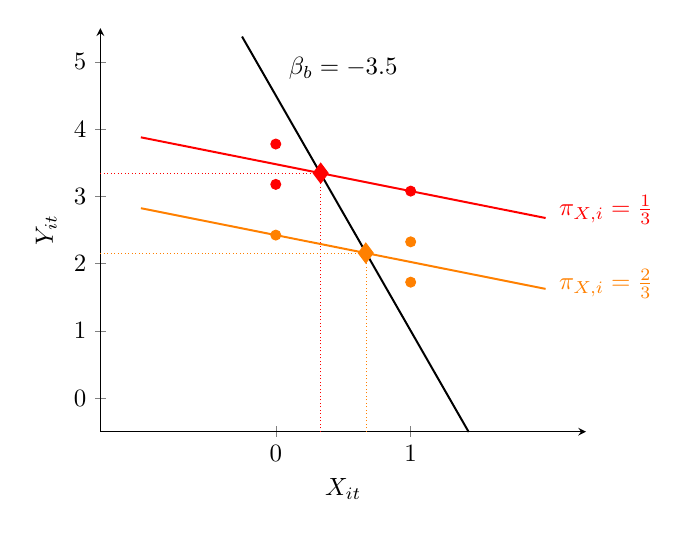
\begin{tikzpicture}[scale=0.9]
                \begin{axis}[
                    axis x line=left, 
                    axis y line=left, 
                    xlabel={$X_{it}$}, ylabel={$Y_{it}$},
                    xmin=-1, xmax=2, ymin=0, ymax=5,
                    xtick={0,1},
                    ytick={0,1,2,3,4,5},
                    enlargelimits=true,
                    clip=false,
                    xshift=-15mm,
                    samples=200,
                    domain=-1:2,
                ]
            
                \pgfmathsetmacro{\gammaZero}{4.5}
                \pgfmathsetmacro{\gammaOne}{-3.1}
                \pgfmathsetmacro{\betaOne}{-0.4}
                \pgfmathsetmacro{\betaB}{-3.5}
            
                % === Person with mu_X = 0.33 ===
                \pgfmathsetmacro{\muXone}{0.33}
                \pgfmathsetmacro{\intOne}{\gammaZero + \gammaOne*\muXone}
                \addplot[thick, red] coordinates {
                    (-1, {\intOne + \betaOne*-1})
                    (2, {\intOne + \betaOne*2})
                };
                \addplot[only marks, mark=diamond*, mark size=4pt, red] coordinates {
                (0.333, {\intOne + \betaOne*0.333})
                };
                \addplot[only marks, red] coordinates {
                    % (0, {\intOne + \betaOne*0})
                    (0, {\intOne + \betaOne*0.75})
                    (0, {\intOne + \betaOne*-0.75})
                    % (1, {\intOne + \betaOne*0.25})
                    (1, {\intOne + \betaOne*1})
                    % (1, {\intOne + \betaOne*1.75})
                };
                \addplot[densely dotted, thin, red] coordinates {
                    (\muXone, -0.5)
                    (\muXone, {\gammaZero + \betaB*\muXone})
                };
                \addplot[densely dotted, thin, red] coordinates {
                    (-1.3, {\gammaZero + \betaB*\muXone})
                    (\muXone, {\gammaZero + \betaB*\muXone})
                };
            
                % === Person with mu_X = 0.67 ===
                \pgfmathsetmacro{\muXtwo}{0.67}
                \pgfmathsetmacro{\intTwo}{\gammaZero + \gammaOne*\muXtwo}
                \addplot[thick, orange] coordinates {
                    (-1, {\intTwo + \betaOne*-1})
                    (2, {\intTwo + \betaOne*2})
                };
                \addplot[only marks, mark=diamond*, mark size=4pt, orange] coordinates {
                (0.667, {\intTwo + \betaOne*0.667})
                };
                \addplot[only marks, orange] coordinates {
                    (0, {\intTwo + \betaOne*0})
                    % (0, {\intTwo + \betaOne*0.75})
                    % (0, {\intTwo + \betaOne*-0.75})
                    (1, {\intTwo + \betaOne*0.25})
                    % (1, {\intTwo + \betaOne*1})
                    (1, {\intTwo + \betaOne*1.75})
                };
                \addplot[densely dotted, thin, orange] coordinates {
                    (\muXtwo, -0.5)
                    (\muXtwo, {\gammaZero + \betaB*\muXtwo})
                };
                \addplot[densely dotted, thin, orange] coordinates {
                    (-1.3, {\gammaZero + \betaB*\muXtwo})
                    (\muXtwo, {\gammaZero + \betaB*\muXtwo})
                };
            
                % === Between-person regression line ===
                \addplot[thick, black, domain=-0.25:1.43] {\gammaZero + \betaB*x};
            
                % === Labels ===
                \node[red] at (axis cs:2.45,2.8) {$\pi_{X,i}=\frac{1}{3}$};
                \node[orange] at (axis cs:2.45,1.7) {$\pi_{X,i}=\frac{2}{3}$};
                \node[black] at (axis cs:0.5,4.9) {$\beta_\text{b} = -3.5$};
            
                \end{axis}
            \end{tikzpicture}
            
            \caption{Binary X and Continuous Y}\label{fig:withinbetween-binxconty}
        \end{subfigure}
    \end{minipage}

    \vskip 1em

    % Bottom row
    \begin{minipage}[t]{.45\linewidth}
        \centering
        \begin{subfigure}[b]{\linewidth}
            \centering

            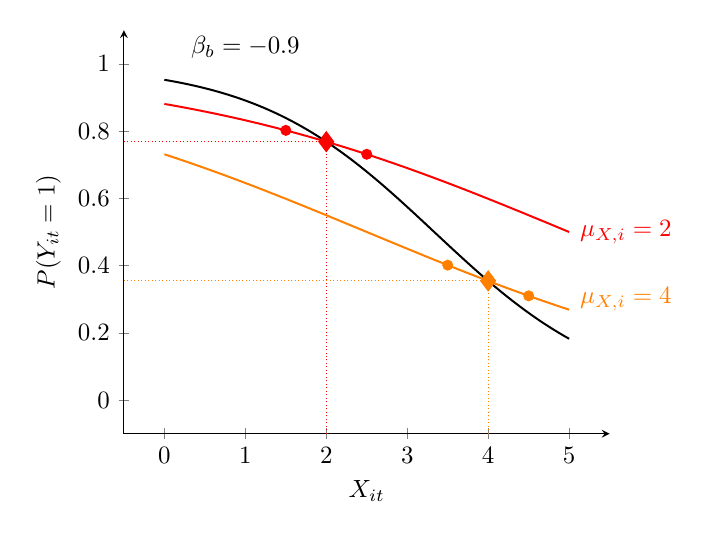
\begin{tikzpicture}[scale=0.9]
            \begin{axis}[
                axis x line=left, axis y line=left,
                xlabel={$X_{it}$}, ylabel={$P(Y_{it} = 1)$},
                xmin=0, xmax=5, ymin=0, ymax=1,
                % legend pos=south west,
                samples=200,
                domain=0:5,
                ytick={0,0.2,0.4,0.6,0.8,1},
                xtick={0,1,2,3,4,5},
                clip=false,
                enlargelimits=true
            ]
            
            % Parameters
            \pgfmathsetmacro{\gammaZero}{3}
            \pgfmathsetmacro{\gammaOne}{-0.5}
            \pgfmathsetmacro{\betaOne}{-0.4}
            \pgfmathsetmacro{\betaB}{-0.9}
            
            % Person 1: mu_X = 2
            \pgfmathsetmacro{\muXone}{2}
            \pgfmathsetmacro{\intOne}{\gammaZero + \gammaOne*\muXone}
            \addplot[red, thick] {1 / (1 + exp(-(\intOne + \betaOne*x)))};
            \addplot[only marks, mark=*, red] coordinates {
                (1.5, {1 / (1 + exp(-(\intOne + \betaOne*1.5)))})
                (2.5, {1 / (1 + exp(-(\intOne + \betaOne*2.5)))})
            };
            \addplot[only marks, mark=diamond*, mark size=4pt, red] coordinates {
                (2, {1 / (1 + exp(-(\intOne + \betaOne*2)))})
            };
            \addplot[densely dotted, thin, red] coordinates {
                (\muXone, -0.1)
                (\muXone, {1 / (1 + exp(-(\intOne + \betaOne*\muXone)))})
            };
            \addplot[densely dotted, thin, red] coordinates {
                (-0.5, {1 / (1 + exp(-(\intOne + \betaOne*\muXone)))})
                (\muXone, {1 / (1 + exp(-(\intOne + \betaOne*\muXone)))})
            };
            
            
            % Person 2: mu_X = 4
            \pgfmathsetmacro{\muXtwo}{4}
            \pgfmathsetmacro{\intTwo}{\gammaZero + \gammaOne*\muXtwo}
            \addplot[orange, thick] {1 / (1 + exp(-(\intTwo + \betaOne*x)))};
            \addplot[only marks, mark=*, orange] coordinates {
                (3.5, {1 / (1 + exp(-(\intTwo + \betaOne*3.5)))})
                (4.5, {1 / (1 + exp(-(\intTwo + \betaOne*4.5)))})
            };
            \addplot[only marks, mark=diamond*, mark size=4pt, orange] coordinates {
                (4, {1 / (1 + exp(-(\intTwo + \betaOne*4)))})
            };
            \addplot[densely dotted, thin, orange] coordinates {
            (\muXtwo, -0.1)
            (\muXtwo, {1 / (1 + exp(-(\intTwo + \betaOne*\muXtwo)))})
            };
            \addplot[densely dotted, thin, orange] coordinates {
            (-0.5, {1 / (1 + exp(-(\intTwo + \betaOne*\muXtwo)))})
            (\muXtwo, {1 / (1 + exp(-(\intTwo + \betaOne*\muXtwo)))})
            };
            
            % Between-person curve
            \addplot[black, thick] {1 / (1 + exp(-(\gammaZero + \betaB*x)))};
        
            % === Labels ===
            \node[red] at (axis cs:5.7,0.5) {$\mu_{X,i}=2$};
            \node[orange] at (axis cs:5.7,0.3) {$\mu_{X,i}=4$};
            \node[black] at (axis cs:1,1.05) {$\beta_\text{b} = -0.9$};
            
            
            \end{axis}
            \end{tikzpicture}
        
            \caption{Continuous X and Binary Y}\label{fig:withinbetween-contxbiny}
        \end{subfigure}
    \end{minipage}
    \hfill
    \begin{minipage}[t]{.45\linewidth}
        \centering
        \begin{subfigure}[b]{\linewidth}
            \centering
            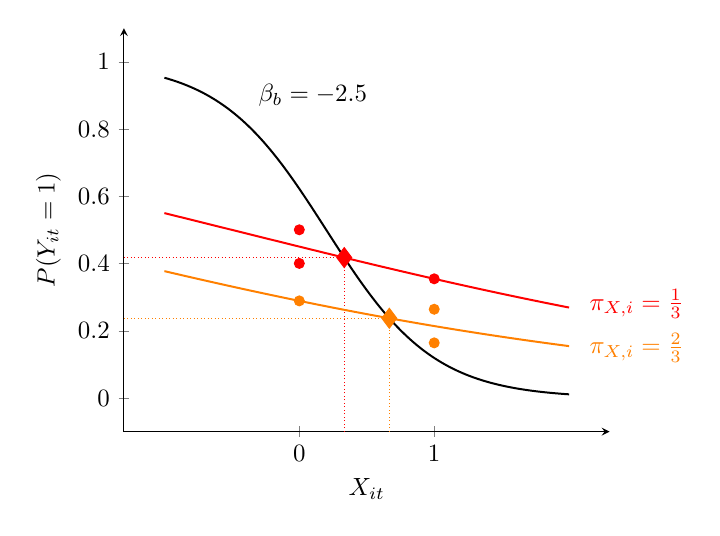
\begin{tikzpicture}[scale=0.9]
            \begin{axis}[
                axis x line=left, axis y line=left,
                xlabel={$X_{it}$}, ylabel={$P(Y_{it} = 1)$},
                xmin=-1, xmax=2, ymin=0, ymax=1,
                % legend pos=south west,
                samples=200,
                domain=-1:2,
                ytick={0,0.2,0.4,0.6,0.8,1},
                xtick={0,1},
                clip=false,
                enlargelimits=true
            ]
            
            % Parameters
            \pgfmathsetmacro{\gammaZero}{0.5}
            \pgfmathsetmacro{\gammaOne}{-2.1}
            \pgfmathsetmacro{\betaOne}{-0.4}
            \pgfmathsetmacro{\betaB}{-2.5}
            
            % Person 1: mu_X = 0.333
            \pgfmathsetmacro{\muXone}{0.333}
            \pgfmathsetmacro{\intOne}{\gammaZero + \gammaOne*\muXone}
            \addplot[red, thick] {1 / (1 + exp(-(\intOne + \betaOne*x)))};
            \addplot[only marks, mark=diamond*, mark size=4pt, red] coordinates {
                (0.333, {1 / (1 + exp(-(\intOne + \betaOne*0.333)))})
            };
            \addplot[only marks, mark=*, red] coordinates {
                % (0, {1 / (1 + exp(-(\intOne + \betaOne*0)))})
                (0, {1 / (1 + exp(-(\intOne + \betaOne*0))) + 0.05})
                (0, {1 / (1 + exp(-(\intOne + \betaOne*0))) - 0.05})
                (1, {1 / (1 + exp(-(\intOne + \betaOne*1)))})
                % (1, {1 / (1 + exp(-(\intOne + \betaOne*1))) + 0.05})
                % (1, {1 / (1 + exp(-(\intOne + \betaOne*1))) - 0.05})
            };
            \addplot[densely dotted, thin, red] coordinates {
                (\muXone, -0.1)
                (\muXone, {1 / (1 + exp(-(\intOne + \betaOne*\muXone)))})
            };
            \addplot[densely dotted, thin, red] coordinates {
                (-1.3, {1 / (1 + exp(-(\intOne + \betaOne*\muXone)))})
                (\muXone, {1 / (1 + exp(-(\intOne + \betaOne*\muXone)))})
            };
            
            % Person 2: mu_X = 0.667
            \pgfmathsetmacro{\muXtwo}{0.667}
            \pgfmathsetmacro{\intTwo}{\gammaZero + \gammaOne*\muXtwo}
            \addplot[orange, thick] {1 / (1 + exp(-(\intTwo + \betaOne*x)))};
            \addplot[only marks, mark=diamond*, mark size=4pt, orange] coordinates {
                (0.667, {1 / (1 + exp(-(\intTwo + \betaOne*0.667)))})
            };
            \addplot[only marks, mark=*, orange] coordinates {
                (0, {1 / (1 + exp(-(\intTwo + \betaOne*0)))})
                % (0, {1 / (1 + exp(-(\intTwo + \betaOne*0))) + 0.05})
                % (0, {1 / (1 + exp(-(\intTwo + \betaOne*0))) - 0.05})
                % (1, {1 / (1 + exp(-(\intTwo + \betaOne*1)))})
                (1, {1 / (1 + exp(-(\intTwo + \betaOne*1))) + 0.05})
                (1, {1 / (1 + exp(-(\intTwo + \betaOne*1))) - 0.05})
            };
            
            \addplot[densely dotted, thin, orange] coordinates {
            (\muXtwo, -0.1)
            (\muXtwo, {1 / (1 + exp(-(\intTwo + \betaOne*\muXtwo)))})
            };
            \addplot[densely dotted, thin, orange] coordinates {
            (-1.3, {1 / (1 + exp(-(\intTwo + \betaOne*\muXtwo)))})
            (\muXtwo, {1 / (1 + exp(-(\intTwo + \betaOne*\muXtwo)))})
            };
            
            % Between-person curve
            \addplot[black, thick] {1 / (1 + exp(-(\gammaZero + \betaB*x)))};
        
            % === Labels ===
            \node[red] at (axis cs:2.5,0.28){$\pi_{X,i}=\frac{1}{3}$};
            \node[orange] at (axis cs:2.5,0.15) {$\pi_{X,i}=\frac{2}{3}$};
            \node[black] at (axis cs:0.1,0.9) {$\beta_\text{b} = -2.5$};
            
            \end{axis}
        \end{tikzpicture}
        \caption{Binary X and Y}\label{fig:withinbetween-binxy}
        \end{subfigure}
    \end{minipage}
    
    \label{fig:path2}

    \vspace{-1cm}
    \begin{flushleft}
    \begin{figurenote}
    Within-person effects ($\beta_1$) and between-person effects ($\beta_b$) are shown for data-generating mechanisms varying by predictor type $X$ (columns) and outcome type $Y$ (rows), each either continuous or binary. For continuous outcomes, relationships are linear; for binary outcomes, the Y-axis reflects the probability of $Y = 1$, and relationships follow a logistic curve. The solid black line denotes the between-person effect; colored lines represent within-person effects for two individuals. Circles are hypothetical observations; diamonds mark where each within-person slope intersects the between-person slope. Thin dotted lines indicate each person's mean on $X$ and $Y$.
    
    % The within-person effects $\beta_1$ and between-person effects $\beta_\text{b}$ illustrated for data-generating mechanisms that vary by predictor type $X$ (columns) and outcome type $Y$ (rows), each either continuous or binary. For continuous outcomes, the relationship between $X$ and $Y$ are linear, whereas for binary outcomes the Y-axis represents a probability of scoring 1, where the effects have a logistic curves.
    % The solid black line represents the \textit{between-person} effect, while the colored solid lines indicate \textit{within-person} effects for two individuals. Circles represent hypothetical observations. Diamonds mark the point where each individual's within-person slope intersects with the between-person slope, and the thin colored dotted lines indicate that individual’s average on on $X$ and on $Y$.
    \end{figurenote}
    \end{flushleft}
\end{center}

% \begin{center}
%     \captionof{figure}{Within- and Between-Person Effects in Data Generating Models with $\beta_\text{w} = -0.4$}
%     % Top row
%     \begin{minipage}[t]{.45\linewidth}
%         \centering
%         \begin{subfigure}[b]{\linewidth}
%             \centering
%             \begin{tikzpicture}
%                 \begin{axis}[
%                     axis x line=left, 
%                     axis y line=left, 
%                     xlabel={$X_{it}$}, ylabel={$Y_{it}$},
%                     xmin=0, xmax=5, ymin=0, ymax=5,
%                     xtick={0,1,2,3,4,5},
%                     ytick={0,1,2,3,4,5},
%                     enlargelimits=true,
%                     clip=false,
%                     xshift=-15mm
%                 ]
            
%                 \pgfmathsetmacro{\gammaZero}{4.5}
%                 \pgfmathsetmacro{\gammaOne}{-0.5}
%                 \pgfmathsetmacro{\betaOne}{-0.4}
%                 \pgfmathsetmacro{\betaB}{-0.9}  % gamma01 + beta1
            
%                 % === Within-person: mu_X = 2 ===
%                 \addplot[domain=0:5, thick, red] {\gammaZero + \gammaOne*2 + \betaOne*x};
%                 \addplot[only marks, red] coordinates {
%                     (1.5, {4.5 - 0.5*2 - 0.4*1.5})
%                     % (2.0, {4.5 - 0.5*2 - 0.4*2.0})
%                     (2.5, {4.5 - 0.5*2 - 0.4*2.5})
%                 };
%                 \addplot[only marks, mark=diamond*, mark size=4pt, red] coordinates {
%                     (2.0, {4.5 - 0.5*2 - 0.4*2.0})
%                 };
%                 \addplot[densely dotted, thin, red] coordinates {
%                     (2.0, -0.5)
%                     (2.0, {4.5 - 0.5*2 - 0.4*2.0})
%                 };
%                 \addplot[densely dotted, thin, red] coordinates {
%                     (-0.5, {4.5 - 0.5*2 - 0.4*2.0})
%                     (2.0, {4.5 - 0.5*2 - 0.4*2.0})
%                 };
            
%                 % === Within-person: mu_X = 4 ===
%                 \addplot[domain=0:5, thick, orange] {\gammaZero + \gammaOne*4 + \betaOne*x};
%                 \addplot[only marks, orange] coordinates {
%                     (3.5, {4.5 - 0.5*4 - 0.4*3.5})
%                     % (4.0, {4.5 - 0.5*4 - 0.4*4.0})
%                     (4.5, {4.5 - 0.5*4 - 0.4*4.5})
%                 };
%                 \addplot[only marks, mark=diamond*, mark size=4pt, orange] coordinates {
%                     (4.0, {4.5 - 0.5*4 - 0.4*4.0})
%                 };
%                 \addplot[densely dotted, thin, orange] coordinates {
%                     (4.0, -0.5)
%                     (4.0, {4.5 - 0.5*4 - 0.4*4.0})
%                 };
%                 \addplot[densely dotted, thin, orange] coordinates {
%                     (-0.5, {4.5 - 0.5*4 - 0.4*4})
%                     (4.0, {4.5 - 0.5*4 - 0.4*4.0})
%                 };
            
%                 % === Between-person regression line ===
%                 \addplot[thick, black, domain=0:5] {\gammaZero + \betaB*x};
            
%                 % === Labels ===
%                 \node[red] at (axis cs:5.7,1.5) {$\mu_{X,i}=2$};
%                 \node[orange] at (axis cs:5.7,0.5) {$\mu_{X,i}=4$};
%                 \node[black] at (axis cs:1.2,4.5) {$\beta_\text{b} = -0.9$};
            
%                 \end{axis}
%             \end{tikzpicture}
%             \caption{Continuous X and Y}\label{fig:withinbetween-contxy}
%         \end{subfigure}
%     \end{minipage}
%     \hfill
%     \begin{minipage}[t]{.45\linewidth}
%         \centering
%         \begin{subfigure}[b]{\linewidth}
%             \centering
%             \begin{tikzpicture}
%             \begin{axis}[
%                 axis x line=left, axis y line=left,
%                 xlabel={$X_{it}$}, ylabel={$P(Y_{it} = 1)$},
%                 xmin=0, xmax=5, ymin=0, ymax=1,
%                 % legend pos=south west,
%                 samples=200,
%                 domain=0:5,
%                 ytick={0,0.2,0.4,0.6,0.8,1},
%                 xtick={0,1,2,3,4,5},
%                 clip=false,
%                 enlargelimits=true
%             ]
            
%             % Parameters
%             \pgfmathsetmacro{\gammaZero}{3}
%             \pgfmathsetmacro{\gammaOne}{-0.5}
%             \pgfmathsetmacro{\betaOne}{-0.4}
%             \pgfmathsetmacro{\betaB}{-0.9}
            
%             % Person 1: mu_X = 2
%             \pgfmathsetmacro{\muXone}{2}
%             \pgfmathsetmacro{\intOne}{\gammaZero + \gammaOne*\muXone}
%             \addplot[red, thick] {1 / (1 + exp(-(\intOne + \betaOne*x)))};
%             \addplot[only marks, mark=*, red] coordinates {
%                 (1.5, {1 / (1 + exp(-(\intOne + \betaOne*1.5)))})
%                 (2.5, {1 / (1 + exp(-(\intOne + \betaOne*2.5)))})
%             };
%             \addplot[only marks, mark=diamond*, mark size=4pt, red] coordinates {
%                 (2, {1 / (1 + exp(-(\intOne + \betaOne*2)))})
%             };
%             \addplot[densely dotted, thin, red] coordinates {
%                 (\muXone, -0.1)
%                 (\muXone, {1 / (1 + exp(-(\intOne + \betaOne*\muXone)))})
%             };
%             \addplot[densely dotted, thin, red] coordinates {
%                 (-0.5, {1 / (1 + exp(-(\intOne + \betaOne*\muXone)))})
%                 (\muXone, {1 / (1 + exp(-(\intOne + \betaOne*\muXone)))})
%             };
            
            
%             % Person 2: mu_X = 4
%             \pgfmathsetmacro{\muXtwo}{4}
%             \pgfmathsetmacro{\intTwo}{\gammaZero + \gammaOne*\muXtwo}
%             \addplot[orange, thick] {1 / (1 + exp(-(\intTwo + \betaOne*x)))};
%             \addplot[only marks, mark=*, orange] coordinates {
%                 (3.5, {1 / (1 + exp(-(\intTwo + \betaOne*3.5)))})
%                 (4.5, {1 / (1 + exp(-(\intTwo + \betaOne*4.5)))})
%             };
%             \addplot[only marks, mark=diamond*, mark size=4pt, orange] coordinates {
%                 (4, {1 / (1 + exp(-(\intTwo + \betaOne*4)))})
%             };
%             \addplot[densely dotted, thin, orange] coordinates {
%             (\muXtwo, -0.1)
%             (\muXtwo, {1 / (1 + exp(-(\intTwo + \betaOne*\muXtwo)))})
%             };
%             \addplot[densely dotted, thin, orange] coordinates {
%             (-0.5, {1 / (1 + exp(-(\intTwo + \betaOne*\muXtwo)))})
%             (\muXtwo, {1 / (1 + exp(-(\intTwo + \betaOne*\muXtwo)))})
%             };
            
%             % Between-person curve
%             \addplot[black, thick] {1 / (1 + exp(-(\gammaZero + \betaB*x)))};
        
%             % === Labels ===
%             \node[red] at (axis cs:5.7,0.5) {$\mu_{X,i}=2$};
%             \node[orange] at (axis cs:5.7,0.3) {$\mu_{X,i}=4$};
%             \node[black] at (axis cs:1,1.05) {$\beta_\text{b} = -0.9$};
            
            
%             \end{axis}
%         \end{tikzpicture}
%             \caption{Continuous X and Binary Y}\label{fig:withinbetween-contxbiny}
%         \end{subfigure}
%     \end{minipage}

%     \vskip 1em

%     % Bottom row
%     \begin{minipage}[t]{.45\linewidth}
%         \centering
%         \begin{subfigure}[b]{\linewidth}
%             \centering
%             \begin{tikzpicture}
%                 \begin{axis}[
%                     axis x line=left, 
%                     axis y line=left, 
%                     xlabel={$X_{it}$}, ylabel={$Y_{it}$},
%                     xmin=-1, xmax=2, ymin=0, ymax=5,
%                     xtick={0,1},
%                     ytick={0,1,2,3,4,5},
%                     enlargelimits=true,
%                     clip=false,
%                     xshift=-15mm,
%                     samples=200,
%                     domain=-1:2,
%                 ]
            
%                 \pgfmathsetmacro{\gammaZero}{4.5}
%                 \pgfmathsetmacro{\gammaOne}{-3.1}
%                 \pgfmathsetmacro{\betaOne}{-0.4}
%                 \pgfmathsetmacro{\betaB}{-3.5}
            
%                 % === Person with mu_X = 0.33 ===
%                 \pgfmathsetmacro{\muXone}{0.33}
%                 \pgfmathsetmacro{\intOne}{\gammaZero + \gammaOne*\muXone}
%                 \addplot[thick, red] coordinates {
%                     (-1, {\intOne + \betaOne*-1})
%                     (2, {\intOne + \betaOne*2})
%                 };
%                 \addplot[only marks, mark=diamond*, mark size=4pt, red] coordinates {
%                 (0.333, {\intOne + \betaOne*0.333})
%                 };
%                 \addplot[only marks, red] coordinates {
%                     % (0, {\intOne + \betaOne*0})
%                     (0, {\intOne + \betaOne*0.75})
%                     (0, {\intOne + \betaOne*-0.75})
%                     % (1, {\intOne + \betaOne*0.25})
%                     (1, {\intOne + \betaOne*1})
%                     % (1, {\intOne + \betaOne*1.75})
%                 };
%                 \addplot[densely dotted, thin, red] coordinates {
%                     (\muXone, -0.5)
%                     (\muXone, {\gammaZero + \betaB*\muXone})
%                 };
%                 \addplot[densely dotted, thin, red] coordinates {
%                     (-1.3, {\gammaZero + \betaB*\muXone})
%                     (\muXone, {\gammaZero + \betaB*\muXone})
%                 };
            
%                 % === Person with mu_X = 0.67 ===
%                 \pgfmathsetmacro{\muXtwo}{0.67}
%                 \pgfmathsetmacro{\intTwo}{\gammaZero + \gammaOne*\muXtwo}
%                 \addplot[thick, orange] coordinates {
%                     (-1, {\intTwo + \betaOne*-1})
%                     (2, {\intTwo + \betaOne*2})
%                 };
%                 \addplot[only marks, mark=diamond*, mark size=4pt, orange] coordinates {
%                 (0.667, {\intTwo + \betaOne*0.667})
%                 };
%                 \addplot[only marks, orange] coordinates {
%                     (0, {\intTwo + \betaOne*0})
%                     % (0, {\intTwo + \betaOne*0.75})
%                     % (0, {\intTwo + \betaOne*-0.75})
%                     (1, {\intTwo + \betaOne*0.25})
%                     % (1, {\intTwo + \betaOne*1})
%                     (1, {\intTwo + \betaOne*1.75})
%                 };
%                 \addplot[densely dotted, thin, orange] coordinates {
%                     (\muXtwo, -0.5)
%                     (\muXtwo, {\gammaZero + \betaB*\muXtwo})
%                 };
%                 \addplot[densely dotted, thin, orange] coordinates {
%                     (-1.3, {\gammaZero + \betaB*\muXtwo})
%                     (\muXtwo, {\gammaZero + \betaB*\muXtwo})
%                 };
            
%                 % === Between-person regression line ===
%                 \addplot[thick, black, domain=-0.25:1.43] {\gammaZero + \betaB*x};
            
%                 % === Labels ===
%                 \node[red] at (axis cs:2.45,2.8) {$\pi_{X,i}=\frac{1}{3}$};
%                 \node[orange] at (axis cs:2.45,1.7) {$\pi_{X,i}=\frac{2}{3}$};
%                 \node[black] at (axis cs:0.5,4.9) {$\beta_\text{b} = -3.5$};
            
%                 \end{axis}
%             \end{tikzpicture}
%             \caption{Binary X and Continuous Y}\label{fig:withinbetween-binxconty}
%         \end{subfigure}
%     \end{minipage}
%     \hfill
%     \begin{minipage}[t]{.45\linewidth}
%         \centering
%         \begin{subfigure}[b]{\linewidth}
%             \centering
%             \begin{tikzpicture}
%             \begin{axis}[
%                 axis x line=left, axis y line=left,
%                 xlabel={$X_{it}$}, ylabel={$P(Y_{it} = 1)$},
%                 xmin=-1, xmax=2, ymin=0, ymax=1,
%                 % legend pos=south west,
%                 samples=200,
%                 domain=-1:2,
%                 ytick={0,0.2,0.4,0.6,0.8,1},
%                 xtick={0,1},
%                 clip=false,
%                 enlargelimits=true
%             ]
            
%             % Parameters
%             \pgfmathsetmacro{\gammaZero}{0.5}
%             \pgfmathsetmacro{\gammaOne}{-2.1}
%             \pgfmathsetmacro{\betaOne}{-0.4}
%             \pgfmathsetmacro{\betaB}{-2.5}
            
%             % Person 1: mu_X = 0.333
%             \pgfmathsetmacro{\muXone}{0.333}
%             \pgfmathsetmacro{\intOne}{\gammaZero + \gammaOne*\muXone}
%             \addplot[red, thick] {1 / (1 + exp(-(\intOne + \betaOne*x)))};
%             \addplot[only marks, mark=diamond*, mark size=4pt, red] coordinates {
%                 (0.333, {1 / (1 + exp(-(\intOne + \betaOne*0.333)))})
%             };
%             \addplot[only marks, mark=*, red] coordinates {
%                 % (0, {1 / (1 + exp(-(\intOne + \betaOne*0)))})
%                 (0, {1 / (1 + exp(-(\intOne + \betaOne*0))) + 0.05})
%                 (0, {1 / (1 + exp(-(\intOne + \betaOne*0))) - 0.05})
%                 (1, {1 / (1 + exp(-(\intOne + \betaOne*1)))})
%                 % (1, {1 / (1 + exp(-(\intOne + \betaOne*1))) + 0.05})
%                 % (1, {1 / (1 + exp(-(\intOne + \betaOne*1))) - 0.05})
%             };
%             \addplot[densely dotted, thin, red] coordinates {
%                 (\muXone, -0.1)
%                 (\muXone, {1 / (1 + exp(-(\intOne + \betaOne*\muXone)))})
%             };
%             \addplot[densely dotted, thin, red] coordinates {
%                 (-1.3, {1 / (1 + exp(-(\intOne + \betaOne*\muXone)))})
%                 (\muXone, {1 / (1 + exp(-(\intOne + \betaOne*\muXone)))})
%             };
            
%             % Person 2: mu_X = 0.667
%             \pgfmathsetmacro{\muXtwo}{0.667}
%             \pgfmathsetmacro{\intTwo}{\gammaZero + \gammaOne*\muXtwo}
%             \addplot[orange, thick] {1 / (1 + exp(-(\intTwo + \betaOne*x)))};
%             \addplot[only marks, mark=diamond*, mark size=4pt, orange] coordinates {
%                 (0.667, {1 / (1 + exp(-(\intTwo + \betaOne*0.667)))})
%             };
%             \addplot[only marks, mark=*, orange] coordinates {
%                 (0, {1 / (1 + exp(-(\intTwo + \betaOne*0)))})
%                 % (0, {1 / (1 + exp(-(\intTwo + \betaOne*0))) + 0.05})
%                 % (0, {1 / (1 + exp(-(\intTwo + \betaOne*0))) - 0.05})
%                 % (1, {1 / (1 + exp(-(\intTwo + \betaOne*1)))})
%                 (1, {1 / (1 + exp(-(\intTwo + \betaOne*1))) + 0.05})
%                 (1, {1 / (1 + exp(-(\intTwo + \betaOne*1))) - 0.05})
%             };
            
%             \addplot[densely dotted, thin, orange] coordinates {
%             (\muXtwo, -0.1)
%             (\muXtwo, {1 / (1 + exp(-(\intTwo + \betaOne*\muXtwo)))})
%             };
%             \addplot[densely dotted, thin, orange] coordinates {
%             (-1.3, {1 / (1 + exp(-(\intTwo + \betaOne*\muXtwo)))})
%             (\muXtwo, {1 / (1 + exp(-(\intTwo + \betaOne*\muXtwo)))})
%             };
            
%             % Between-person curve
%             \addplot[black, thick] {1 / (1 + exp(-(\gammaZero + \betaB*x)))};
        
%             % === Labels ===
%             \node[red] at (axis cs:2.5,0.28){$\pi_{X,i}=\frac{1}{3}$};
%             \node[orange] at (axis cs:2.5,0.15) {$\pi_{X,i}=\frac{2}{3}$};
%             \node[black] at (axis cs:0.1,0.9) {$\beta_\text{b} = -2.5$};
            
%             \end{axis}
%         \end{tikzpicture}
%         \caption{Binary X and Y}\label{fig:withinbetween-binxy}
%         \end{subfigure}
%     \end{minipage}
    
%     \label{fig:path2}

%     % \vspace{-2cm}
%     \begin{flushleft}
%     \begin{figurenote}
%     The solid black line represents the \textit{between-person} effect, while the colored solid lines indicate \textit{within-person} effects for each individual. Circles represent hypothetical observations. Diamonds mark the point where each individual's within-person slope intersects with the between-person slope, and the thin colored dotted lines indicate that individual’s average on on $X$ and on $Y$.
%     \end{figurenote}
%     \end{flushleft}
% \end{center}


\subsection{DGM 2: Binary Predictor and Continuous Outcome}


% Here, \( Z_i \) follows the same distribution as \( \mu_{X,i} \) in Equation~\ref{eqn:xbetweencontxy}.

To illustrate the DGM for a binary predictor and continuous outcome, we consider the case where daily engagement in a mindfulness practice (e.g., meditation), coded as 1 if practiced and 0 otherwise, predicts experiences of anger (see Figure~\ref{fig:path-binxconty}). Each individual is characterized by a latent propensity to engage in mindfulness on a given day, denoted \( Z_i \), which varies across individuals according to a normal distribution \( Z_i \sim \mathcal{N}(0, \sigma^2_{X,\text{b}}) \), identical to \( \mu_{X,i} \) in DGM 1. This continuous latent trait is transformed via a logistic function to yield the individual-specific probability \( \pi_{X,i} \in (0,1) \) of engaging in mindfulness, with values ranging from 0 to 1:
\begin{align}
    \pi_{X,i} &= \frac{e^{Z_i}}{1+ e^{Z_i}}
\end{align}
The observed binary predictor $X$ for individual $i$ at occasion $t$,  denoted \( X_{it} \in \{0,1\} \), is a combination of the underlying probability \( \pi_{X,i} \) and fluctuations in the Bernoulli sampling process $X_{it} \sim \text{Bernoulli}(\pi_{X,i})$. In this way, each person’s binary predictor values vary across time due to probabilistic sampling, and the extent of within-person variability is a function of their underlying propensity \( \pi_{X,i} \). Individuals with extreme probabilities (close to 0 or 1) will show little within-person variation, whereas those with moderate probabilities exhibit more fluctuation.

Anger on day \( t \) for person \( i \), denoted \( Y_{it} \), is modeled as a function of both between- and within-person components of mindfulness engagement. The within-person equation is the same as in DGM 1 (see equation~\ref{eqn:yit-generationmlm}). The between-person equation now takes the form:  
\begin{equation}
    \label{eqn:dgm2-betweenlevel}
    \beta_{0i} = \gamma_{00} + \gamma_{01} \pi_{X,i} + u_{0i},
\end{equation}
with \( \gamma_{00} \) representing the grand mean of anger, \( \gamma_{01} \) the contextual effect of average mindfulness engagement, and \( u_{0i} \sim \mathcal{N}(0, \sigma^2_u) \) capturing person-level heterogeneity unexplained by \( \pi_{X,i} \). Substituting this into the within-person model yields the composite model:
\begin{equation}
    Y_{it} = \gamma_{00} + \gamma_{01} \pi_{X,i} + u_{0i} + \beta_1 X_{it} + e_{it}.
\end{equation}
This DGM captures two distinct effects of mindfulness practice (\( X \)) on anger (\( Y \)). The within-person effect \( \beta_1 \) reflects how anger changes on days with versus without mindfulness practice, so that \( \beta_1 = \beta_{\text{w}}\). The contextual effect \( \gamma_{01} \) captures whether individuals who typically engage more in mindfulness experience systematically different anger levels than expected based on their day-to-day engagement alone. 

To reflect the plausible scenario in which mindfulness engagement has a stronger effect between persons than within persons, we may specify $\gamma_{00} = 4.5, \quad \gamma_{01} = -3.1, \quad \beta_1 = -0.4$ resulting in a between-person effect of \( \beta_\text{b} = -3.5 \). This pattern, visualized in Figure~\ref{fig:withinbetween-binxconty}, suggests that individuals who engage in mindfulness more frequently benefit from reduced anger not solely explained by their day-to-day practice—indicating a trait-level or contextual benefit. As in DGM 1, the two individuals differ only with regard tot their random intercept $\beta_{0i}$. The person with the orange line has a greater overall probability of practicing mindfulness ($\pi_{X,i} = \frac{2}{3}$) than the person with the red line ($\pi_{X,i} = \frac{1}{3}$). Considering that the between-level effect of $X$ on $Y$ is negative, this means that the person with the orange line also has lower overall anger than the person with the red line.

% \begin{center}
    \captionof{figure}{Within- and Between-Person Effects of Binary Predictor and Continuous Outcome}

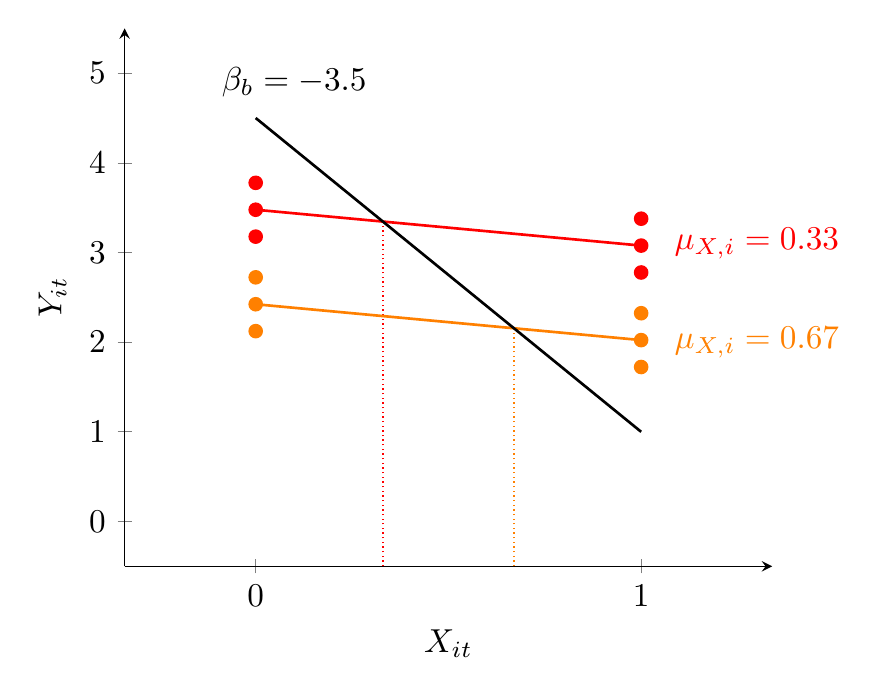
\begin{tikzpicture}[scale=1.2]
    \begin{axis}[
        axis x line=left, 
        axis y line=left, 
        xlabel={$X_{it}$}, ylabel={$Y_{it}$},
        xmin=-0.2, xmax=1.2, ymin=0, ymax=5,
        xtick={0,1},
        ytick={0,1,2,3,4,5},
        enlargelimits=true,
        clip=false,
        xshift=-15mm
    ]

    \pgfmathsetmacro{\gammaZero}{4.5}
    \pgfmathsetmacro{\gammaOne}{-3.1}
    \pgfmathsetmacro{\betaOne}{-0.4}
    \pgfmathsetmacro{\betaB}{-3.5}

    % === Person with mu_X = 0.33 ===
    \pgfmathsetmacro{\muXone}{0.33}
    \pgfmathsetmacro{\intOne}{\gammaZero + \gammaOne*\muXone}
    \addplot[thick, red] coordinates {
        (0, {\intOne + \betaOne*0})
        (1, {\intOne + \betaOne*1})
    };
    \addplot[only marks, red] coordinates {
        (0, {\intOne + \betaOne*0})
        (0, {\intOne + \betaOne*0.75})
        (0, {\intOne + \betaOne*-0.75})
        (1, {\intOne + \betaOne*0.25})
        (1, {\intOne + \betaOne*1})
        (1, {\intOne + \betaOne*1.75})
    };
    \addplot[densely dotted, thin, red] coordinates {
        (\muXone, -0.5)
        (\muXone, {\gammaZero + \betaB*\muXone})
    };

    % === Person with mu_X = 0.67 ===
    \pgfmathsetmacro{\muXtwo}{0.67}
    \pgfmathsetmacro{\intTwo}{\gammaZero + \gammaOne*\muXtwo}
    \addplot[thick, orange] coordinates {
        (0, {\intTwo + \betaOne*0})
        (1, {\intTwo + \betaOne*1})
    };
    \addplot[only marks, orange] coordinates {
        (0, {\intTwo + \betaOne*0})
        (0, {\intTwo + \betaOne*0.75})
        (0, {\intTwo + \betaOne*-0.75})
        (1, {\intTwo + \betaOne*0.25})
        (1, {\intTwo + \betaOne*1})
        (1, {\intTwo + \betaOne*1.75})
    };
    \addplot[densely dotted, thin, orange] coordinates {
        (\muXtwo, -0.5)
        (\muXtwo, {\gammaZero + \betaB*\muXtwo})
    };

    % === Between-person regression line ===
    \addplot[thick, black, domain=0:1] {\gammaZero + \betaB*x};

    % === Labels ===
    \node[red] at (axis cs:1.3,3.1) {$\mu_{X,i}=0.33$};
    \node[orange] at (axis cs:1.3,2.0) {$\mu_{X,i}=0.67$};
    \node[black] at (axis cs:0.1,4.9) {$\beta_\text{b} = -3.5$};

    \end{axis}
\end{tikzpicture}

    \label{fig:withinbetween-binxconty}
    \begin{figurenote}
        The solid black slope represents the between-person effect and the colored slopes the within-cluster effects. The X-axis simultaneously represents $X_{it}$ for the within-slope and $\mu_{X,i}$ for the between-slope; and the Y-axis represents $Y_{it}$ for the within slope and $Y_i$ for the between-slope. Dots reflect possible datapoints and diamonds reflect the position of $\mu_{X,i}$ on the within-person slope.
    \end{figurenote}
\end{center}

\subsection{DGM 3: Continuous Predictor and Binary Outcome}

To illustrate the DGM for a continuous predictor and a binary outcome, we consider how daily levels of mindfulness relate to the probability of experiencing an anger episode, coded as 1 if an anger episode occured and 0 otherwise (see Figure~\ref{fig:path-contxbiny}). The coninuous predictor $X_{it}$ is generated as described in DGM 1 (see equation~\ref{eqn:relationwithinmundlak}). The binary outcome \( Y_{it} \in \{0, 1\} \) reflects whether an anger episode occurred for person $i$ on day \( t \). Rather than modeling \( Y_{it} \) directly at the within-level, we model its probability using the logistic link:
\begin{equation}
    \label{eqn:logitwi}
    \text{logit}(P(Y_{it} = 1)) = \beta_{0i} + \beta_1 X_{it},
\end{equation}
The between-level equation is the same as in DGM 1 (see equation~\ref{eqn:beta0-generationcontxy}). Substituting the between-person equation into the within-person model yields the full generative model:
\begin{equation}
\text{logit}(P(Y_{it} = 1)) = \gamma_{00} + \gamma_{01} \mu_{X,i} + u_{0i} + \beta_1 X_{it}.
\end{equation}
The fixed effects have the same interpretation as in DGM 1, but now represent effects on the log-odds scale. Accordingly, the within-person effect \( \beta_1 = \beta_{\text{w}} \) reflects how daily deviations in mindfulness relate to changes in the \textit{log-odds} of experiencing anger. The contextual effect \( \gamma_{01} \) captures the extent to which trait mindfulness relates to the baseline log-odds of anger beyond the within-person effect.
    
To specify a plausible generative structure, we might assume \( \gamma_{00} = 3, \gamma_{01} = -0.5, \beta_1 = -0.4 \), so that the between-person effect \( \beta_\text{b} = -0.9 \). This pattern, visualized in Figure~\ref{fig:withinbetween-contxbiny}, reflects that individuals with higher average mindfulness are less likely to experience anger episodes, beyond what is expected from daily fluctuations alone. While we now have a logistic curve instead of a linear line as in DGM 1 and 2, the within-person effect remains identical for the two individuals. The difference between the individuals pertains only to the random intercept $\beta_{0i}$. The person with the orange line has datapoints clustered around a greater trait-level of mindfulness ($\mu_{X,i} = 4$) than the person with the red line ($\mu_{X,i} = 2$). Due to the negative between-person effect of $X$ on $Y$, it follows that the person with the orange line also has lower overall probability of experiencing an anger episode.

% \begin{center}
    \captionof{figure}{Within- and Between-Person Effects of Continuous Predictor and Binary Outcome}

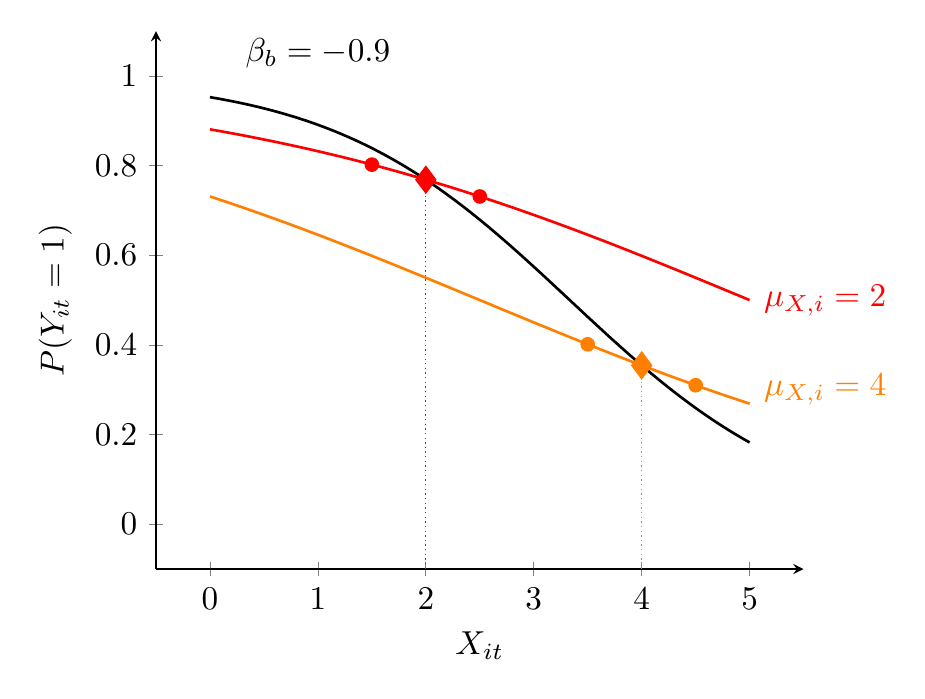
\begin{tikzpicture}[scale=1.2]
    \begin{axis}[
        axis x line=left, axis y line=left,
        xlabel={$X_{it}$}, ylabel={$P(Y_{it} = 1)$},
        xmin=0, xmax=5, ymin=0, ymax=1,
        % legend pos=south west,
        samples=200,
        domain=0:5,
        ytick={0,0.2,0.4,0.6,0.8,1},
        xtick={0,1,2,3,4,5},
        clip=false,
        enlargelimits=true
    ]
    
    % Parameters
    \pgfmathsetmacro{\gammaZero}{3}
    \pgfmathsetmacro{\gammaOne}{-0.5}
    \pgfmathsetmacro{\betaOne}{-0.4}
    \pgfmathsetmacro{\betaB}{-0.9}
    
    % Person 1: mu_X = 2
    \pgfmathsetmacro{\muXone}{2}
    \pgfmathsetmacro{\intOne}{\gammaZero + \gammaOne*\muXone}
    \addplot[red, thick] {1 / (1 + exp(-(\intOne + \betaOne*x)))};
    \addplot[only marks, mark=*, red] coordinates {
        (1.5, {1 / (1 + exp(-(\intOne + \betaOne*1.5)))})
        (2.5, {1 / (1 + exp(-(\intOne + \betaOne*2.5)))})
    };
    \addplot[only marks, mark=diamond*, mark size=4pt, red] coordinates {
        (2, {1 / (1 + exp(-(\intOne + \betaOne*2)))})
    };
    \addplot[densely dotted, thin, red] coordinates {
        (\muXone, -0.1)
        (\muXone, {1 / (1 + exp(-(\intOne + \betaOne*\muXone)))})
    };
    
    
    % Person 2: mu_X = 4
    \pgfmathsetmacro{\muXtwo}{4}
    \pgfmathsetmacro{\intTwo}{\gammaZero + \gammaOne*\muXtwo}
    \addplot[orange, thick] {1 / (1 + exp(-(\intTwo + \betaOne*x)))};
    \addplot[only marks, mark=*, orange] coordinates {
        (3.5, {1 / (1 + exp(-(\intTwo + \betaOne*3.5)))})
        (4.5, {1 / (1 + exp(-(\intTwo + \betaOne*4.5)))})
    };
    \addplot[only marks, mark=diamond*, mark size=4pt, orange] coordinates {
        (4, {1 / (1 + exp(-(\intTwo + \betaOne*4)))})
    };
    \addplot[densely dotted, thin, orange] coordinates {
    (\muXtwo, -0.1)
    (\muXtwo, {1 / (1 + exp(-(\intTwo + \betaOne*\muXtwo)))})
    };
    
    % Between-person curve
    \addplot[black, thick] {1 / (1 + exp(-(\gammaZero + \betaB*x)))};

    % === Labels ===
    \node[red] at (axis cs:5.7,0.5) {$\mu_{X,i}=2$};
    \node[orange] at (axis cs:5.7,0.3) {$\mu_{X,i}=4$};
    \node[black] at (axis cs:1,1.05) {$\beta_\text{b} = -0.9$};
    
    
    \end{axis}
\end{tikzpicture}

    \label{fig:withinbetween-contxbiny}
    \begin{figurenote}
        The solid black slope represents the between-person effect and the colored slopes the within-cluster effects. The X-axis simultaneously represents $X_{it}$ for the within-slope and $\mu_{X,i}$ for the between-slope; and the Y-axis represents $Y_{it}$ for the within slope and $Y_i$ for the between-slope. Dots reflect possible datapoints and diamonds reflect the position of $\mu_{X,i}$ on the within-person slope.
    \end{figurenote}
\end{center}

\subsection{DGM 4: Binary Predictor and Outcome}

To illustrate the DGM for a binary predictor and a binary outcome, we consider how engaging in a mindfulness practice (1 = yes, 0 = no) relates to the probability of experiencing an anger episode (1 = yes, 0 = no) on the same day (see Figure~\ref{fig:path-binxy}). The predictor \( X_{it} \) and the person-specific probability $\pi_{X,i}$ are generated as described in DGM 2. 

Anger episode on day \( t \) for person \( i \), denoted \( Y_{it} \), is modeled as a function of both between- and within-person components of mindfulness engagement. The within-person equation is the same as in DGM 3 (see equation~\ref{eqn:logitwi}) and the between-person equation is the same as in DGM 2 (see equation~\ref{eqn:dgm2-betweenlevel}). The composite model becomes:
\begin{equation}
    \text{logit}(P(Y_{it} = 1)) = \gamma_{00} + \gamma_{01} \pi_{X,i} + u_{0i} + \beta_1 X_{it}.
\end{equation}
The fixed effects have the same interpretation as in DGM 2, but now represent effects on the log-odds scale as in DGM 3. In this specification, the within-person effect \( \beta_1 = \beta_{\text{w}} \) captures the average change in log-odds of experiencing anger on days with vs. without mindfulness practice, while \( \gamma_{01} \) quantifies how stable engagement in mindfulness practice relates to the likelihood of anger episodes independently of daily fluctuations.

A plausible parameter setting might be \( \gamma_{00} = 0.5, \gamma_{01} = -2.1, \beta_1 = -0.4 \), so that $\beta_\text{b} = -2.5$. As shown in Figure~\ref{fig:withinbetween-binxy}, this means that both stable and situational mindfulness practice reduce the likelihood of anger episodes, and that the contextual effect exceeds the within-person effect. 
As in DGM 3, we now have a logistic curve instead of a linear line as in DGM 1 and 2. Nevertheless, the within-person effect remains identical for the two individuals with the difference between the individuals pertaining only to the random intercept $\beta_{0i}$.  The person with the orange line has a greater overall probability of practicing mindfulness ($\pi_{X,i} = \frac{2}{3}$) than the person with the red line ($\pi_{X,i} = \frac{1}{3}$). Due to the negative between-person effect of $X$ on $Y$, it follows that the person with the orange line also has lower overall probability of experiencing an anger episode.

% \begin{center}
    \captionof{figure}{Within- and Between-Person Effects of Binary Predictor and Outcome}

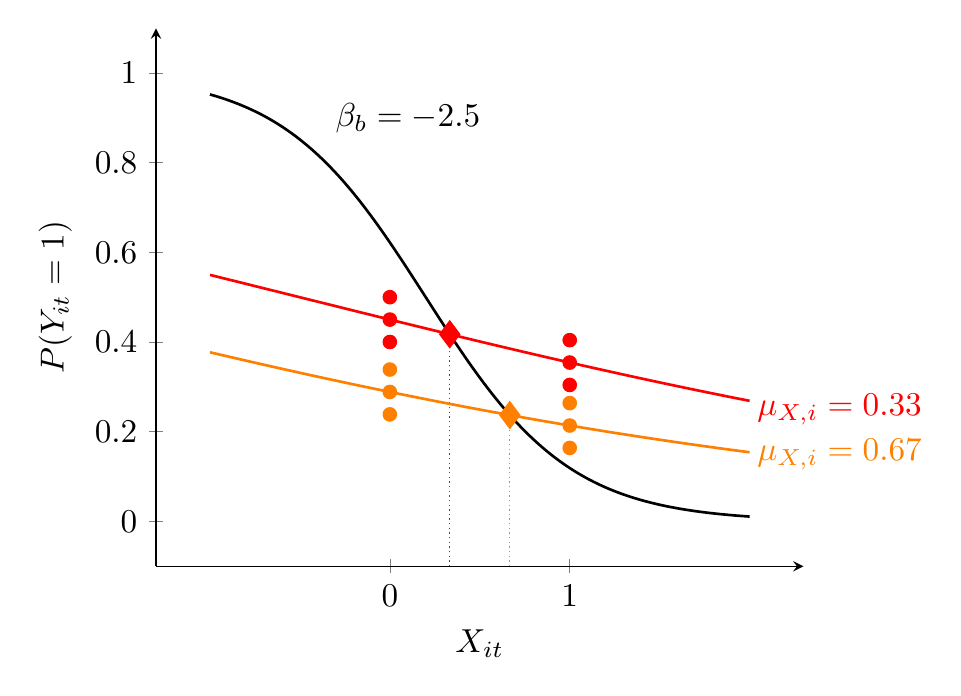
\begin{tikzpicture}[scale=1.2]
    \begin{axis}[
        axis x line=left, axis y line=left,
        xlabel={$X_{it}$}, ylabel={$P(Y_{it} = 1)$},
        xmin=-1, xmax=2, ymin=0, ymax=1,
        % legend pos=south west,
        samples=200,
        domain=-1:2,
        ytick={0,0.2,0.4,0.6,0.8,1},
        xtick={0,1},
        clip=false,
        enlargelimits=true
    ]
    
    % Parameters
    \pgfmathsetmacro{\gammaZero}{0.5}
    \pgfmathsetmacro{\gammaOne}{-2.1}
    \pgfmathsetmacro{\betaOne}{-0.4}
    \pgfmathsetmacro{\betaB}{-2.5}
    
    % Person 1: mu_X = 0.333
    \pgfmathsetmacro{\muXone}{0.333}
    \pgfmathsetmacro{\intOne}{\gammaZero + \gammaOne*\muXone}
    \addplot[red, thick] {1 / (1 + exp(-(\intOne + \betaOne*x)))};
    \addplot[only marks, mark=diamond*, mark size=4pt, red] coordinates {
        (0.333, {1 / (1 + exp(-(\intOne + \betaOne*0.333)))})
    };
    \addplot[only marks, mark=*, red] coordinates {
        (0, {1 / (1 + exp(-(\intOne + \betaOne*0)))})
        (0, {1 / (1 + exp(-(\intOne + \betaOne*0))) + 0.05})
        (0, {1 / (1 + exp(-(\intOne + \betaOne*0))) - 0.05})
        (1, {1 / (1 + exp(-(\intOne + \betaOne*1)))})
        (1, {1 / (1 + exp(-(\intOne + \betaOne*1))) + 0.05})
        (1, {1 / (1 + exp(-(\intOne + \betaOne*1))) - 0.05})
    };
    \addplot[densely dotted, thin, red] coordinates {
        (\muXone, -0.1)
        (\muXone, {1 / (1 + exp(-(\intOne + \betaOne*\muXone)))})
    };
    
    % Person 2: mu_X = 0.667
    \pgfmathsetmacro{\muXtwo}{0.667}
    \pgfmathsetmacro{\intTwo}{\gammaZero + \gammaOne*\muXtwo}
    \addplot[orange, thick] {1 / (1 + exp(-(\intTwo + \betaOne*x)))};
    \addplot[only marks, mark=diamond*, mark size=4pt, orange] coordinates {
        (0.667, {1 / (1 + exp(-(\intTwo + \betaOne*0.667)))})
    };
    \addplot[only marks, mark=*, orange] coordinates {
        (0, {1 / (1 + exp(-(\intTwo + \betaOne*0)))})
        (0, {1 / (1 + exp(-(\intTwo + \betaOne*0))) + 0.05})
        (0, {1 / (1 + exp(-(\intTwo + \betaOne*0))) - 0.05})
        (1, {1 / (1 + exp(-(\intTwo + \betaOne*1)))})
        (1, {1 / (1 + exp(-(\intTwo + \betaOne*1))) + 0.05})
        (1, {1 / (1 + exp(-(\intTwo + \betaOne*1))) - 0.05})
    };
    
    \addplot[densely dotted, thin, orange] coordinates {
    (\muXtwo, -0.1)
    (\muXtwo, {1 / (1 + exp(-(\intTwo + \betaOne*\muXtwo)))})
    };
    
    % Between-person curve
    \addplot[black, thick] {1 / (1 + exp(-(\gammaZero + \betaB*x)))};

    % === Labels ===
    \node[red] at (axis cs:2.5,0.25){$\mu_{X,i}=0.33$};
    \node[orange] at (axis cs:2.5,0.15) {$\mu_{X,i}=0.67$};
    \node[black] at (axis cs:0.1,0.9) {$\beta_\text{b} = -2.5$};
    
    \end{axis}
\end{tikzpicture}

    \label{fig:withinbetween-binxy}
    \begin{figurenote}
        The solid black slope represents the between-person effect and the colored slopes the within-cluster effects. The X-axis simultaneously represents $X_{it}$ for the within-slope and $\mu_{X,i}$ for the between-slope; and the Y-axis represents $Y_{it}$ for the within slope and $Y_i$ for the between-slope. Dots reflect possible datapoints and diamonds reflect the position of $\mu_{X,i}$ on the within-person slope.
    \end{figurenote}
\end{center}

 % The intercept \( \gamma_{00} \) represents the expected log-odds of interpersonal conflict for an individual who never engages in mindfulness ($\pi_{X,i} = 0$) . The within-person effect \( \beta_1 \) quantifies how an individual's likelihood of experiencing conflict changes on days when they engage in mindfulness practice versus days when they do not. The contextual effect \( \gamma_{01} \) captures the degree to which the between-person effect---the association between a person's long-term tendency to engage in mindfulness \( \pi_{X,i} \) and their overall tendency to experience conflict---differs from the within-person effect. The between-person effect $\beta_\text{b} = \gamma_{01} + \beta_\text{w}$ describes whether individuals who generally engage in mindfulness more frequently experience a systematically different likelihood of being involved in conflict compared to those who rarely or never engage in the practice.  

\section{Modeling Frameworks}

To analyze the hierarchical longitudinal data generated by the specified DGMs, we adopt two primary modeling frameworks: GLMMs and GEE. Within the GLMM framework, we employ both a standard MLM for continuous outcomes and a multilevel logistic model for binary outcomes. Within the GEE framework, we consider three commonly used implementations that differ in their specification of the working correlation matrix.

We consider four methods of disentangling the within-person and between-person slopes. We first formalize these methods within an MLM with a continuous predictor for analysis of DGM 1, offering a clear reference point. We then extend this discussion to binary predictors for analysis of DGM 2. Following this, we introduce the multilevel logistic model for analysis of DGM 3 and 4 and demonstrate how the four disaggregation methods are implemented in this context. Finally, we turn to the GEE framework, detailing how each method can be adapted to estimate within- and between-person effects under different working correlation structures.

% Contextual effects—differences in the predictor–outcome relationship across levels—are central to this issue. Within- and between-subject associations often differ substantially in magnitude and may even have opposite signs. Ignoring this distinction can lead to conceptual errors, notably the ecological fallacy: the mistaken inference that relationships observed at the between-cluster level necessarily hold at the within-cluster level \parencite{robinson_ecological_1950, bolger_intensive_2013}.

\subsection{Generalized Linear Multilevel Model}

The GLMM extends the Generalized Linear Model (GLM) to accommodate hierarchical or clustered data structures. Like the GLM, the GLMM allows the analyst to specify an appropriate distribution for the outcome variable (e.g., normal, binomial, Poisson) and a link function that defines the relationship between the linear predictor and the expected outcome. However, unlike the GLM, which assumes independence of observations, the GLMM explicitly accounts for dependence among observations within clusters—such as repeated measures within individuals—by incorporating random effects.

This modeling framework generalizes the classical MLM by permitting non-normal outcomes and non-identity link functions, thereby broadening its applicability to a wide range of data types. In this paper, we focus on two widely used instantiations of the GLMM: (1) the MLM which is a special case of the GLMM with a normally distributed outcome and an identity link function and (2) the multilevel logistic model which is a GLMM with a binary outcome, modeled using a binomial distribution and a logit link function.

\subsubsection{Multilevel Linear Model}

In MLM, it is well established that when using continuous, time-varying predictors, researchers must distinguish within-person effects from between-person effects. This distinction is critical because a model that does not explicitly separate these sources of variation will produce a conflated estimate that mixes the two, impairing interpretability and potentially leading to incorrect conclusions \parencite[e.g.,][]{enders_centering_2007, kreft_effect_1995, raudenbush_hierarchical_2002}.

This concern is especially relevant when the within-cluster (i.e., person-level) effect is the primary target of inference or causal interpretation. If the within- and between-person associations are identical—or if only one of them is present—there is no conflation and bias is absent. However, in typical psychological research, one cannot assume that contextual effects are absent as level-specific effects can differ drastically \parencite[]{curran_disaggregation_2011, robinson_ecological_1950}. In fact, detecting and modeling such contextual effects is often one of the key motivations for applying MLMs.

\paragraph{Uncentered Predictor}

Consider that we fit the following simple two-level model to DGM 1 with a time-varying predictor \( X_{it} \) and a random intercept:
\begin{align}
\label{eqn:method-M1-linear-within}
Y_{it} &= \beta_{0i} + \beta_1 X_{it} + e_{it}, \\
\label{eqn:method-M1-linear-between}
\beta_{0i} &= \gamma_{00} + u_{0i}.
\end{align}
Substituting the between-person equation into the within-level model yields:
\begin{equation}
\label{eqn:method-M1-linear}
Y_{it} = \gamma_{00} + u_{0i} + \beta_1 X_{it} + e_{it}.
\end{equation}
In this formulation, the estimate of \( \beta_1 \) reflects a blend of the within-person and between-person associations. The degree to which each component contributes to the estimate depends on the number of time points per individual (\( T \)) and the amount of variability at each level \parencite{mundlak_pooling_1978}. As \( T \) increases, the estimate tends to be more influenced by the within-person effect, but the conflation remains unless explicitly modeled.

The source of this conflation can be understood by considering a causal path diagram (see Figure~\ref{fig:path-contxy}), where the latent mean of the predictor \( \mu_X  \), serves as a common cause of both \( X_{it} \) and \( Y_{it} \) (via its influence on the random intercept \( \beta_{0i} \)). In other words, \( \mu_X \) acts as a confounder in the relationship between \( X_{it} \) and \( Y_{it} \). This confounding disappears under two special cases: (1) when there is no contextual effect (i.e., the path from \( \mu_X \) to the outcome is zero), or (2) when there is no between-person variation in \( \mu_X \) (i.e., all individuals have the same stable latent mean predictor value). Outside of these conditions, failing to account for \( \mu_X \) results in biased estimation of the within-person effect.

To obtain unbiased and interpretable estimates of both within- and between-person effects, several methods have been proposed. We review and compare four such methods in this study.

\paragraph{Within-Person Centered Predictor}

One solution is centering the predictor $X$ within clusters, yielding the cluster mean $\bar{X_i}$ and the within-person centered predictor $(X_{it} - \bar{X_i})$. This method ensures that the within-person slope is not confounded by between-person differences \parencite[e.g.,][]{hoffman_longitudinal_2015, kreft_effect_1995, raudenbush_hierarchical_2002}. The model is then specified as:
\begin{align}
Y_{it} &= \beta_{0i} + \beta_\text{w} (X_{it}- \bar{X_i}) + e_{it},  \\
\beta_{0i} &= \gamma_{00} + u_{0i}.
\end{align}
Substituting the second equation into the first gives:
\begin{equation}
\label{eqn:method-M2-linear}
Y_{it} = \gamma_{00} + u_{0i} + \beta_\text{w} (X_{it}- \bar{X_i}) + e_{it}.
\end{equation}
Since $(X_{it} - \bar{X_i})$ contains no between-person variance, $\beta_\text{w}$ estimates the within-person slope. To obtain the between-person slope $\beta_\text{b}$, the cluster mean $\bar{X_i}$ is added as a predictor:
\begin{align}
\beta_{0i} &= \gamma_{00} + \beta_\text{b} \bar{X_i} + u_{0i}.
\end{align}
The full model then becomes:
\begin{equation}
\label{eqn:method-M4-linear}
Y_{it} = \gamma_{00} + \beta_\text{b} \bar{X_i} + u_{0i} + \beta_\text{w} (X_{it} - \bar{X_i}) + e_{it}.
\end{equation}
\paragraph{Mundlak's Contextual Model}

An alternative approach, known as Mundlak's model \parencite{mundlak_pooling_1978}, retains the raw predictor $X_{it}$ in the within-person equation while including $\bar{X_i}$ in the between-person equation:
\begin{align}
Y_{it} &= \beta_{0i} + \beta_\text{w} X_{it} + e_{it}, \\
\beta_{0i} &= \gamma_{00} + \gamma_{01} \bar{X_i} + u_{0i}.
\end{align}
Substituting the second equation into the first gives:
\begin{equation}
\label{eqn:method-M3-linear}
Y_{it} = \gamma_{00} + \gamma_{01} \bar{X_i} + u_{0i} + \beta_\text{w} X_{it} + e_{it}.
\end{equation}
At first glance, it may seem unintuitive that the regression coefficient for the raw, uncentered time-varying predictor \( X_{it} \) in a model that includes the person-mean \( \bar{X}_i \) represents the within-person effect. However, this result follows from the statistical relationship between \( X_{it} \) and \( \bar{X}_i \) (see equation~\ref{eqn:relationwithinmundlak}), which are inherently correlated \parencite[cf.][]{hoffman_longitudinal_2015}. When both terms are included in the model, their shared variance in predicting the outcome is partialled out, and each coefficient reflects its unique contribution. Specifically, the coefficient for \( X_{it} \) captures the within-person effect \( \beta_\text{w} \) and the coefficient for \( \bar{X}_i \), in turn, captures the contextual effect \( \gamma_{01} \). Given the absence of random slope and no interactions between  \( X_{it} \) and \( \bar{X}_i \), the contextual effect is given by \( \gamma_{01} = \beta_\text{b} - \beta_\text{w} \) and the between-person effect can be computed as  \(   \beta_\text{b} = \gamma_{01} +  \beta_\text{w}\) \parencite{raudenbush_hierarchical_2002}.

\paragraph{Disaggregation Methods for Binary Predictors}

Although binary predictors differ substantively from continuous variables, the statistical principles underlying their treatment in MLMs are analogous. As shown by \textcite{enders_centering_2007}, the algebra and logic of centering does not require us to distinguish between continuous and categorical predictors.\footnote{See \textcite{yaremych_centering_2023} for a discussion on the importance of centering (multi)categorical predictors.} Consequently, the same four disaggregation methods used for continuous predictors can be applied to binary predictor in DGM 2 without modification. However, the application of methods has distinct interpretational implications when involving binary compared to continuous predictors.

For binary predictors, the cluster mean \( \bar{X}_i \) is an estimate of $\pi_{X,i}$ and represents the proportion of time the event occurs for individual \( i \) (e.g., the proportion of days on which the person engaged in mindfulness). The person-mean centered term \( X_{it} - \bar{X}_i \) thus reflects momentary deviations from this personal base rate. Accordingly, the within-person slope \( \beta_\text{w} \) captures how changes in event status (e.g., practicing mindfulness vs. not) at a specific timepoint are associated with changes in the outcome within individuals (e.g., reductions in anger on days with mindfulness practice). In contrast, the between-person slope \( \beta_\text{b} \) quantifies how individual differences in the overall event frequency (e.g., proportion of days with practice) relate to average differences in the outcome across individuals. As in the continuous case, the contextual effect \( \gamma_{01} \) represents the discrepancy between these two associations $\gamma_{01} = \beta_\text{b} - \beta_\text{w}$ under specific conditions.

However, working with binary predictors introduces practical challenges. When an individual’s event probability \( \bar{X}_i \) is close to 0 or 1, there is limited within-person variability, which can yield unstable estimates of \( \beta_\text{w} \). Additionally, with few measurement occasions (\( T \)), the number of unique values \( \bar{X}_i \) can take is limited to \( T + 1 \) discrete levels. For instance, with \( T = 5 \), the only possible values of \( \bar{X}_i \) are 0.00, 0.20, 0.40, 0.60, 0.80, and 1.00. This coarseness in the between-person predictor may limit the precision of \( \beta_\text{b} \).

\subsubsection{Multilevel Logistic Model}

When the outcome variable is binary (e.g., experiencing an anger episode), a linear model is no longer appropriate due to the bounded nature of probabilities (between 0 and 1). To analyze such data structures—such as those generated in DGM 3 and 4—we employ the multilevel logistic model, a specific form of the Generalized Linear Mixed Model (GLMM) using a binomial distribution and a logit link function \parencite{anderson_variance_1985, stiratelli_random-effects_1984}.

\paragraph{The Logit Link and Interpretation of Effects}

In logistic models, the linear predictor maps onto the probability of a binary event via the logit function:
\[
\text{logit}(p) = \log\left(\frac{p}{1 - p}\right),
\]
which transforms probabilities \( p \in (0, 1) \) onto the unbounded log-odds scale \( (-\infty, \infty) \). As a consequence, the parameters and partition of variance do not have the intuitive interpretation familiar from linear models \parencite{merlo_brief_2006}. Fixed effects describe changes in log-odds rather than in the outcome variable itself. For interpretability, log-odds can be converted back into probabilities using the inverse logit transformation:
\[
p = \frac{e^{\eta}}{1 + e^{\eta}}, \quad \text{where } \eta \text{ is the linear predictor}.
\]
As in MLMs for continuous outcomes, fixed effects in multilevel logistic have an interpretation that is \textit{conditional} on the random effects. These conditional or 'subject-specific' coefficients reflect changes at the individual level, holding the random effect---in this case $u_{0i}$---constant. In practice, this means that we interpret coefficients as the change in log-odds of an outcome for a unit change in the exposure, for the average individual (at $u_{0i} = 0$ as we assume that $u_{0i}$ is distributed normally with mean zero). Such conditional interpretations are particularly desirable when the inferential focus is on person-level change, which is often the primary goal in longitudinal psychological research.

To explain how disaggregation applies in this context, we revisit the four models introduced in the linear case and illustrate them using DGM 3 (continuous predictor). The same logic generalizes to DGM 4 (binary predictor).

\paragraph{Uncentered Predictor}

We begin with a model including the raw predictor:
\begin{equation}
    \label{eqn:M1-logit}
\text{logit}(\Pr(Y_{it} = 1)) = \gamma_{00} + u_{0i} + \beta_1 X_{it}.
\end{equation}
Here, \( \beta_1 \) reflects a conflated estimate conditional on $u_{0i}$ combining within- and between-person components. As with the MLM, this estimate lacks a clear interpretation unless both effects coincide or one is absent.

\paragraph{Within-Person Centered Predictor}

To isolate the within-person effect, we center the predictor around the individual’s mean:
\begin{equation}
    \label{eqn:M2-logit}
\text{logit}(\Pr(Y_{it} = 1)) = \gamma_{00} + u_{0i} + \beta_\text{w} (X_{it} - \bar{X}_i).
\end{equation}
Now, \( \beta_\text{w} \) captures the effect of deviations from a person’s own average conditional on $u_{0i}$. To also obtain an estimate of the bewteen-person effect, we include the cluster mean:
\begin{equation}
    \label{eqn:M4-logit}
\text{logit}(\Pr(Y_{it} = 1)) = \gamma_{00} + \beta_\text{b} \bar{X}_i + u_{0i} + \beta_\text{w} (X_{it} - \bar{X}_i).
\end{equation}
This formulation allows \( \beta_\text{w} \) to represent the within-person effect and \( \beta_\text{b} \) the between-person effect—how typical levels of the predictor relate to overall likelihood of the outcome given $u_{0i}$.

\paragraph{Mundlak's Contextual Model}

An equivalent model formulation includes both the raw predictor and its person-mean:
\begin{equation}
    \label{eqn:M3-logit}
\text{logit}(\Pr(Y_{it} = 1)) = \gamma_{00} + \gamma_{01} \bar{X}_i + u_{0i} + \beta_\text{w} X_{it}.
\end{equation}
This is algebraically equivalent to the previous model, with the between-person effect recovered as \( \beta_\text{b} = \gamma_{01} + \beta_\text{w} \). 

\paragraph{Practical Example}

To concretize these interpretations, we fit Mundlak's contextual model to DGM 3, where we find the following estimates: \( \gamma_{00} = 3 \), \( \gamma_{01} = -0.5 \), and \( \beta_\text{w} = -0.4 \), implying a total between-person effect \( \beta_\text{b} = -0.9 \). This scenario is visualized in Figure~\ref{fig:withinbetween-contxbiny}. Filling these estimates in equation \ref{eqn:M3-logit} gives:
\[
\text{logit}(P(Y_{it} = 1)) = 3 - 0.9 \bar{X}_i - 0.4 (X_{it} - \bar{X}_i) + u_{0i}.
\]
Let us first consider the within-person effect. Suppose Clara has an average mindfulness score of \( \bar{X}_i = 2 \), and on a given day scores \( X_{it} = 2 \) (i.e., at her mean). For the average person (\( u_{0i} = 0 \)), the log-odds of an anger episode are:
\[
\text{logit}(P(Y_{it} = 1)) = 3 - 0.9 \cdot 2 = 1.2,
\]
which corresponds to:
\[
P(Y_{it} = 1) = \frac{e^{1.2}}{1 + e^{1.2}} \approx 0.77.
\]
Now suppose Clara scores one point above her average (i.e., \( X_{it} = 3 \)). Then:
\[
\text{logit}(P(Y_{it} = 1)) = 1.2 - 0.4 = 0.8,
\]
\[
P(Y_{it} = 1) \approx \frac{e^{0.8}}{1 + e^{0.8}} \approx 0.69.
\]
Thus, a one-unit increase in mindfulness relative to her usual level decreases the probability of an anger episode from 77\% to 69\%, illustrating the within-person effect. Let us now consider the between-person effect Now consider Clara (\( \bar{X}_i = 2 \)) and Maya (\( \bar{X}_i = 4 \)), both at their respective means (\( X_{it} = \bar{X}_i \)). For Maya:
\[
\text{logit}(P(Y_{it} = 1)) = 3 - 0.9 \cdot 4 = -0.6,
\]
\[
P(Y_{it} = 1) \approx \frac{e^{-0.6}}{1 + e^{-0.6}} \approx 0.35.
\]
Although both are at their own typical mindfulness level, Maya’s higher average score results in a much lower anger probability than Clara’s (35\% vs. 77\%). This reflects the between-person effect of mindfulness: individuals with higher typical mindfulness experience anger episodes less frequently overall.

\subsection{Generalized Estimating Equations}

GEE were introduced by \textcite{liang_longitudinal_1986} as an extension of GLMs for analyzing correlated, non-normally distributed outcomes—most notably, longitudinal and clustered data. Coefficients estimated with GEE will be akin to those estimated with (linear or logistic) regression, but standard errors will be adjusted for dependency. Unlike GLMMs, the most common GEE approaches do not include random effects. Instead, they account for within-cluster correlation through a so-called \textit{working correlation structure}. Since GEE do not model random effects, they make fewer unverifiable assumptions, which can be beneficial in applied settings \parencite[]{mcneish_unnecessary_2017, hubbard_gee_2010}.

GEE are often referred to as \textit{marginal models} because they estimate population-averaged effects \parencite{diggle_analysis_2002}. In GEE, the interpretation of a coefficient mirrors that of a standard GLM: the expected change in the mean outcome for a one-unit change in the predictor, \textit{averaged across the entire population}. In contrast, models that include random effects—such as GLMMs—yield conditional or \textit{cluster-specific} estimates: the expected change in the outcome for a one-unit increase in the predictor, \textit{holding the random effect constant}, which typically corresponds to inference for the “average” individual (i.e., assuming the random intercept \( u_{0i} = 0 \)).

A central distinction between GEE and GLMMs emerges when the link function is nonlinear (e.g., logit). While both frameworks converge to similar interpretations under an identity link and continuous outcome—where the fixed effect coefficients represent both conditional (within-cluster) and marginal (population-averaged) effects—this equivalence breaks down with nonlinear links \parencite[]{neuhaus_comparison_1991}.\footnote{An interactive RShiny app illustrating the relationship between marginal and conditional effects in multilevel logistic models can be found at: \href{https://wardeiling.shinyapps.io/GLMM_population-averaged-and-person-specific-interpretations/}{https://wardeiling.shinyapps.io/GLMM\_population-averaged-and-person-specific-interpretations/}.} Thus, with a logit link, GLMMs deliver conditional estimates and GEEs deliver marginal estimates, making the choice of model central to how binary outcome parameters are interpreted. While approximations exist for converting cluster-specific effects to marginal effects \parencite[cf.][]{austin_intermediate_2017}, they rely on distributional assumptions.

Importantly, whether a marginal or conditional interpretation is preferable depends on the scientific aim of the study. Consider the example of a longitudinal study examining the effect of mindfulness on the occurrence of anger episodes (a binary outcome). A marginal question suitable for GEE might be: ``How does practicing mindfulness affect the overall likelihood of experiencing anger episodes in the general population?'' Here, the focus is on population-average effects, such as informing public health interventions. A conditional question suitable for GLMM might be: ``For a given individual, how does their likelihood of experiencing an anger episode change following an increase in mindfulness?'' Here, the focus is on understanding within-person processes and making inferences about individual trajectories.

To account for within-cluster correlation, GEE require specification of a working correlation structure \( R \) that encodes the expected correlation \( \rho \) among repeated measurements \( Y_{it} \) within cluster \( i \). Common choices include the independence, exchangeable, and first-order autoregressive (AR(1)) structures. The \textit{independence} structure assumes no within-cluster correlation and is often used as a baseline:
\[
R = 
\begin{bmatrix}
1 & 0 & 0 & 0 & 0 \\
0 & 1 & 0 & 0 & 0 \\
0 & 0 & 1 & 0 & 0 \\
0 & 0 & 0 & 1 & 0 \\
0 & 0 & 0 & 0 & 1
\end{bmatrix}
\]
The \textit{exchangeable} structure assumes constant correlation between all pairs of measurements within a cluster:
\[
R = 
\begin{bmatrix}
1 & \rho & \rho & \rho & \rho \\
\rho & 1 & \rho & \rho & \rho \\
\rho & \rho & 1 & \rho & \rho \\
\rho & \rho & \rho & 1 & \rho \\
\rho & \rho & \rho & \rho & 1
\end{bmatrix}
\]
The \textit{AR(1)} structure assumes that correlations decay exponentially with increasing time lag, which is often appropriate for regularly spaced longitudinal data:
\[
R = 
\begin{bmatrix}
1 & \rho & \rho^2 & \rho^3 & \rho^4 \\
\rho & 1 & \rho & \rho^2 & \rho^3 \\
\rho^2 & \rho & 1 & \rho & \rho^2 \\
\rho^3 & \rho^2 & \rho & 1 & \rho \\
\rho^4 & \rho^3 & \rho^2 & \rho & 1
\end{bmatrix}
\]
While correctly specifying the working correlation can improve efficiency, GEE estimates tend to remain consistent even under misspecification \parencite{zeger_models_1988, ballinger_using_2004}.

GEE estimation is based on iterative quasi-likelihood rather than full maximum likelihood, as in GLMMs. This makes convergence criteria less straightforward\footnote{The convergence criterion in GEE relies on the stabilization of estimating functions rather than likelihood gradients \parencite[p. 92]{hardin_generalized_2012}.} and complicates procedures such as likelihood-based model comparison. For an accessible introduction to the computational and practical aspects of GEE—including the iterative estimation procedure and considerations for model selection—see \textcite{mcneish_unnecessary_2017} and \textcite{ballinger_using_2004}.

\paragraph{Disaggregation Methods and GEE}

Disaggregation methods can, in principle, be applied within the GEE framework by removing the random intercept term \( u_{0i} \) from GLMM equations. For continuous outcomes, this entails using MLM equations with an identity link; for binary outcomes, multilevel logistic model equations with a logit link are adapted accordingly. Although it is technically possible to specify GEE models in this manner, the conceptual interpretation of within-person and contextual effects under GEE remains unclear. For continuous outcomes, where marginal and conditional associations coincide, GEE-based disaggregation is expected to yield estimates similar to those from MLMs, and applying disaggregation methods may be appropriate when the within-person or contextual effects are the targets of inference. However, for binary outcomes with a logit link, GEE estimates must be interpreted marginally \parencite{neuhaus_comparison_1991}. This is problematic since the notions of within-person effects (typically conditional) and population-averaged effects (marginal) may be fundamentally incompatible. To our knowledge, no empirical or theoretical work has systematically examined the role of within-person, between-person, or contextual effects within the GEE framework.

\section{Simulation Study}

The aim of this simulation study is twofold. First, to evaluate whether standard modeling practices for handling contextual effects in MLMs with continuous predictors—such as person-mean centering and inclusion of the cluster mean—generalize to GLMMs with (a) binary predictors and (b) binary outcomes estimated via a logit link function. Second, to investigate whether GEE require an explicit separation of within- and between-person effects through predictor parameterizations in the presence of contextual effects, and to assess the implications of omitting such parameterizations on estimation accuracy and statistical inferences. Specifically, we investigate the impact of different design factors, such as sample size, number of measurement occasions, and variance components, on estimation bias in the fixed within and contextual effects. Simulations and model estimation were conducted in \texttt{R} version 4.4.2 \parencite{r_core_team_r_2024}. Parallel computing was used for efficiency via the \texttt{doFuture} \parencite{RJ-2021-048} and \texttt{foreach} \parencite{daniel_foreach_2022} packages. The codes for simulating and analyzing these data are provided as online supplemental material: INSERT OSF/GITHUB LINK.

\subsection{Data Generation}

Data were simulated as DGM1-4, depending on the measurement level of predictor and outcome. Certain parameters were held constant across all simulation scenarios. The within-cluster standard deviation of $X$ was fixed at $\sigma_{X,\text{w}} = 1$, and the residual variance was set at $\sigma_e = 1$ to maintain a standardized scale for effect sizes. The fixed intercept $\gamma_{00}$ was set to 0 to simplify interpretation. The within-cluster effect $\beta_{\text{w}}$ was fixed at 1.5 to represent a moderate-to-large association, ensuring sufficient signal relative to noise across conditions. We systematically varied key design factors as summarized in Table~\ref{tab:simstudysetup}, excluding scenarios with zero between-person variance but a non-zero contextual effect, which are not meaningful. This resulted in 504 unique simulation conditions. Each condition was replicated 1000 times.

\begin{center}
    \captionof{table}{Summary of Parameters for Each of the Data-Generating Scenarios}
    \label{tab:simstudysetup}
    
    \begin{longtable}{lcc}
    \toprule
    Factor & Notation & Values \\
    \midrule
    Sample size  & \(N_{\text{total}}\) & 100, 200 \\
    Number of time points  & \(T_{\text{total}}\) & 5, 10, 20 \\
    Predictor type  &  & Continuous, Binary\\
    Outcome type  &  & Continuous, Binary\\
    Within-cluster SD in $X$  & \(\sigma_{X,\text{w}}\) & 1 \\
    Between-cluster SD in $X$  & \(\sigma_{X,\text{b}}\) & 0, 1, 3 \\
    Fixed intercept  & \(\gamma_{00}\) & 0 \\
    Contextual effect  & \(\gamma_{01}\) & 0, 1, 3 \\
    Within-cluster effect  & \(\beta_{\text{w}}\) & 1.5 \\
    Random intercept variance (level 2) & \(\sigma_{u0}\) & 0, 1, 3 \\
    Residual variance (level 1)  & \(\sigma_e\) & 1 \\
    \bottomrule
    \end{longtable}
\end{center}

\subsection{Data Analysis}

Each simulated dataset was analyzed using two modeling frameworks: GLMMs and GEE. GLMMs were estimated using the \texttt{lmer} and \texttt{glmer} functions from the \texttt{lme4} package \parencite{bates_fitting_2015} with full maximum likelihood estimation for \texttt{lmer}, as the focus was on fixed effects rather than variance components. GEE models were fitted using the \texttt{geeglm} function from the \texttt{geepack} package \parencite{halekoh_r_2006} under independent, exchangeable, and AR(1) structures. For GEE, the maximum number of iterations was increased from the default 25 to 50 to support convergence. To summarize, as modeling strategies we have GLMM and three implementations of GEE, yielding a total of four modeling strategies.

Each of these four modeling strategies was implemented with four distinct methods. Method 1 is based on the raw predictor $X_{it}$ (i.e., no centering) and is known to yield a slope $\beta$ that is a blend of within- and between-person slopes \parencite[]{raudenbush_hierarchical_2002}. Method 2 uses cluster-mean centering of the predictor and is known to result in an estimate of the within-person slope $\beta_\text{w}$. Method 3 is Munlak's contextual model, which is based on the raw predictor $X_{it}$ with the cluster mean added as a predictor of the random intercept, resulting in estimates of the within-person slope $\beta_\text{w}$ and the contextual effect $\gamma_{01}$. Method 4 uses cluster-mean centering of the predictor and includes the cluster-mean as predictor of the random intercept, yielding an estimate of the within-person slope $\beta_\text{w}$ and between-person slope $\beta_\text{b}$. As method 3 and method 4 yielded consistent results across all scenarios, we decided to present the results of method 3 only.\footnote{Information comparing the two methods are provided as online supplemental material: INSERT OSF/GITHUB LINK.} Considering four modeling strategies with three implementations, we arrive at 12 analysis strategies. We refer to the GLMM implementations with different methods as M1, M2 and M3. Likewise, we refer to GEE implementations as G1, G2 and G3, with the name of the correlation structure appended.

The primary estimates of interest were the within-cluster effect \( \beta_{\text{w}} \) and the contextual effect \( \gamma_{01} \). Model performance was evaluated primarily in terms of estimation bias, calculated as \( \hat{\theta} - \theta \), where \( \hat{\theta} \) is the estimated parameter value and \( \theta \) is the corresponding true population value. When relevant, we also examined convergence rates and estimation efficiency (i.e., variability across replications). All warnings and errors encountered during model estimation were logged. Models failing due to convergence issues or singular fits were excluded from the analysis. Diagnostic checks revealed that parameter estimates from the \texttt{geeglm} function \parencite{halekoh_r_2006} occasionally reached implausibly large magnitudes (e.g., $10^{12}$ or $10^{13}$) when modeling binary outcomes, likely indicative of non-convergence. In instances where an extreme estimate occurred, it exceeded $\pm 10^{11}$, whereas the majority of estimates were tightly clustered within $\pm 2.5$ units around the mean bias. Across 76 simulation scenarios, we observed at least one replication with an estimate exceeding $\pm 10^{11}$. Extreme estimates occurred predominantly in the GEE models using an AR(1) working correlation structure and methods G2 and G3; in one scenario, approximately half of the replications produced extreme values. To maintain the integrity of the reported results, we excluded all estimates exceeding $\pm 10^{11}$ from the final analyses. Results were stored for post-processing and visual inspection.

\subsection{Results}

To facilitate interpretation, we focus on four main scenarios, holding the following constants: \( N = 200 \), \( \sigma_e = 1 \), \( \gamma_{00} = 0 \), \( \beta_{\text{w}} = 1.5 \), \( \gamma_{01} = 3 \),  \(\sigma_{X,\text{w}} = 1\) and \(\sigma_{X,\text{b}} = 3\). We varied \(\sigma_u = \{0, 3\}\) to assess the impact of unexplained heterogeneity, especially on GEE, which does not model random effects; and \( T = \{5, 20\} \) to evaluate performance under limited versus sufficient repeated measures. Sample size \(N\) had a negligible impact on average bias and is not discussed further.

\paragraph{DGM 1: Continuous Predictor and Outcome}

Figure~\ref{fig:dgm1-within} and Figure~\ref{fig:dgm1-contextual} display bias in within-person and contextual effect estimates for benchmark DGM 1. As expected, Method 1 (uncentered predictor) yielded biased within-person estimates across all models, with bias and variability decreasing as \(T\) increased—consistent with the increasing dominance of within-person effect in the composite slope. GEE with an exchangeable correlation (G1-exchangeable) closely mirrored the MLM estimates (M1), the AR(1) structure yielded slightly lower bias (for some other scenarios this was reversed) and the independence structure yielded substantially more bias. In contrast, disaggregation methods (Methods 2 and 3) resulted in tightly distributed unbiased within-person estimates across all frameworks and correlation structures. Contextual effect estimates (Method 3) were similarly unbiased and consistent across MLM and GEE. In summary, all modeling frameworks and correlation structures can recover the within-person and contextual effects well in linear models when predictors and outcomes are continuous and a disaggregation method is applied.

% \begin{center}
%     \captionof{figure}{Bias for DGM 1 in Within-Person and Contextual Effect for Different Estimation Approaches}
%     \begin{subfigure}{0.49\linewidth}
%         \centering
%         
\includegraphics[width=\linewidth, keepaspectratio]{Figures/pred_continuous_out_continuous_bias_plot_T_total-vs-sd.u0_within.pdf}
%         \caption{Within-Person Effect}\label{fig:dgm1-within}
%     \end{subfigure}
%     \hfill
%     \begin{subfigure}{0.49\linewidth}
%         \centering
%         
\includegraphics[height=6, keepaspectratio]{Figures/pred_continuous_out_continuous_bias_plot_T_total-vs-sd.u0_contextual.pdf}
%         \caption{Contextual Effect (Method 3)}\label{fig:dgm1-contextual}
%     \end{subfigure}
%     \label{fig:dgm1}
%     % \begin{figurenote}
%     %     \ldots
%     % \end{figurenote}
% \end{center}

\begin{center}
    \captionof{figure}{Bias for DGM 1 in Within-Person and Contextual Effect for Different Estimation Approaches}
     \hspace*{-1.5cm}
    \begin{subfigure}{0.80\linewidth}  % Set width proportionally for the first figure
        \centering
        
\includegraphics[height=10.6cm, keepaspectratio]{Figures/pred_continuous_out_continuous_bias_plot_T_total-vs-sd.u0_within.pdf}
        \caption{Within-Person Effect $\beta_1$}\label{fig:dgm1-within}
    \end{subfigure}
    \hfill
    \begin{subfigure}{0.25\linewidth}  % Set width proportionally for the second figure
        \centering
        
\includegraphics[height=10.6cm, keepaspectratio]{Figures/pred_continuous_out_continuous_bias_plot_T_total-vs-sd.u0_contextual.pdf}
        \caption{Contextual Effect $\gamma_{01}$ (Method MuCo)}\label{fig:dgm1-contextual}
    \end{subfigure}
    \label{fig:dgm1}
    \begin{flushleft}
        \begin{figurenote}
        The boxplot shows bias based on 1000 replications for data-generating model 1, which includes a continuous predictor and outcome. The boxes represent the interquartile range (IQR) from the 25th to 75th percentiles, with the median indicated by the horizontal line inside. Whiskers extend to 1.5 times the IQR, and replications outside this range are plotted as dots. UC = uncentered, CWC = centered within clusters, MuCo = Mundlak contextual, GLMM = generalized linear mixed model, GEE = generalized estimating equations. $T$ represents the total number of time points, and $\sigma_u$ denotes the random intercept residual variance. Y-axis breaks represent large intervals relative to bias but are consistent across data-generating models. In panel (a), GEE-UC with an independence correlation structure falls outside the plotted range, with estimates tightly clustered around 2.7 across all four scenarios.

        % The boxplot shows bias based on 1000 replications for data-generating model 1, which includes a continuous predictor and outcome. The boxes represent the interquartile range from the 25th to 75th percentiles, with the median indicated by the horizontal line inside. Whiskers extend to 1.5 times the IQR, and replications outside this range are plotted as dots. UC refers to uncentered, CWC to centered within clusters, and MuCo to Mundlak contextual, GLMM to generalized linear mixed model, GEE to generalized estimating equations. $T$ represents the total number of time points, and $\sigma_u$ denotes the random intercept residual variance. Y-axis breaks represent large intervals relative to bias but were chosen to be consistent across data-generating models. In panel (a), GEE-UC with independence correlation structure falls outside the plotted range, with estimates clustered tightly around 2.7 across all four scenarios.
        
        % Bias is shown for for data-generating model 1, which includes a continuous predictor and outcome. UC = uncentered; CWC = centered within clusters; MuCo = Mundlak contextual; $T$ = total number of time points; $\sigma_u$ = random intercept variance. Y-axis breaks represent large intervals relative to bias but were chosen to be consistent across data-generating models. In panel (a), GEE-UC with independence correlation structure falls outside the plotted range, with estimates clustered tightly around 2.7 across all four scenarios.
        
        % UC: Uncentered, CWC: centered within clusters, MuCo: Mundlak Contextual, T: total number of timepoints, $\sigma_u$: the random intercept residual variance. The breaks on the $Y$-axis represent large steps relative to bias, but were chosen to be consistent with the other DGMs. For panel (a), GEE-UC-independence fell outside the bounds, but has estimates tightly clustered around 2.7 (for all four scenarios).
    \end{figurenote}
    \end{flushleft}
\end{center}

% \begin{center}
%     \captionof{figure}{Bias for DGM 1 in Within-Person and Contextual Effect for Different Estimation Approaches}
%     \begin{subfigure}{1.1\linewidth}
%         \centering
%         
\includegraphics[width=\linewidth, keepaspectratio]{Figures/pred_continuous_out_continuous_bias_plot_T_total-vs-sd.u0_within.pdf}
%         \caption{Within-Person Effect}\label{fig:dgm1-within}
%     \end{subfigure}
%     \begin{subfigure}{1.1\linewidth}
%         \centering
%         
\includegraphics[width=\linewidth, keepaspectratio]{Figures/pred_continuous_out_continuous_bias_plot_T_total-vs-sd.u0_contextual.pdf}
%         \caption{Contextual Effect (Method 3)}\label{fig:dgm1-contextual}
%     \end{subfigure}
%     \label{fig:dgm1}
%     % \begin{figurenote}
%     %     \ldots
%     % \end{figurenote}
% \end{center}

\paragraph{DGM 2: Binary Predictor and Continuous Outcome}

Figure~\ref{fig:dgm2} present results for DGM 2. Patterns were very similar to DGM 1, though with increased overall variability, impact of unexplained variability ($\sigma_u$) and more pronounced bias. The findings of Method 1 mirror that of DGM 1. However, unlike DGM 1, greater unexplained heterogeneity (\(\sigma_u = 3\)) reduced bias in Method 1, likely due to an increased ratio of unexplained to explained (between-person) variance in $\beta_{0i}$. As before, disaggregation methods (M2, M3, G2, G3) yielded unbiased within-person estimates. Contextual effect estimates were again robust across models using Method 3. Thus, across frameworks and correlation structures, disaggregation methods effectively recovers the true effects even when predictors are binary.

% \begin{center}
%     \captionof{figure}{Bias for DGM 2 in Within-Person and Contextual Effect for Different Estimation Approaches}
%     \begin{subfigure}{1.1\linewidth}
%         \centering
%         
\includegraphics[width=\linewidth, keepaspectratio]{Figures/pred_binary_out_continuous_bias_plot_T_total-vs-sd.u0_within.pdf}
%         \caption{Within-Person Effect}\label{fig:dgm2-within}
%     \end{subfigure}
%     % \hfill
%     \begin{subfigure}{1.1\linewidth}
%         \centering
%         
\includegraphics[width=\linewidth, keepaspectratio]{Figures/pred_binary_out_continuous_bias_plot_T_total-vs-sd.u0_contextual.pdf}
%         \caption{Contextual Effect (Method 3)}\label{fig:dgm2-contextual}
%     \end{subfigure}
%     \label{fig:dgm2}
%     % \begin{figurenote}
%     %     \ldots
%     % \end{figurenote}
% \end{center}


\begin{center}
    \captionof{figure}{Bias for DGM 2 in Within-Person and Contextual Effect for Different Estimation Approaches}
     \hspace*{-1.5cm}
    \begin{subfigure}{0.80\linewidth}  % Set width proportionally for the first figure
        \centering
        
\includegraphics[height=10.6cm, keepaspectratio]{Figures/pred_binary_out_continuous_bias_plot_T_total-vs-sd.u0_within.pdf}
        \caption{Within-Person Effect $\beta_1$}\label{fig:dgm2-within}
    \end{subfigure}
    \hfill
    \begin{subfigure}{0.25\linewidth}  % Set width proportionally for the second figure
        \centering
        
\includegraphics[height=10.6cm, keepaspectratio]{Figures/pred_binary_out_continuous_bias_plot_T_total-vs-sd.u0_contextual.pdf}
        \caption{Contextual Effect $\gamma_{01}$ (Method MuCo)}\label{fig:dgm2-contextual}
    \end{subfigure}
    \label{fig:dgm2}
    \begin{flushleft}
        \begin{figurenote}
        The boxplot shows bias based on 1000 replications for data-generating model 2, which includes a binary predictor and continuous outcome. The boxes represent the interquartile range (IQR) from the 25th to 75th percentiles, with the median indicated by the horizontal line inside. Whiskers extend to 1.5 times the IQR, and replications outside this range are plotted as dots. UC = uncentered, CWC = centered within clusters, MuCo = Mundlak contextual, GLMM = generalized linear mixed model, GEE = generalized estimating equations. $T$ represents the total number of time points, and $\sigma_u$ denotes the random intercept residual variance.

        
        % The boxplot shows bias based on 1000 replications for data-generating model 2, which includes a binary predictor and continuous outcome. The boxes represent the interquartile range from the 25th to 75th percentiles, with the median indicated by the horizontal line inside. Whiskers extend to 1.5 times the IQR, and points outside this range are considered outliers, plotted as dots. UC refers to uncentered, CWC to centered within clusters, and MuCo to Mundlak contextual. $T$ represents the total number of time points, and $\sigma_u$ denotes the random intercept residual variance.
        % Bias is shown for data-generating model 2, which includes a binary predictor and continuous outcome. UC refers to uncentered, CWC to centered within clusters, and MuCo to Mundlak contextual. $T$ represents the total number of time points, and $\sigma_u$ denotes the random intercept residual variance.
    \end{figurenote}
    \end{flushleft}
\end{center}

\paragraph{DGM 3: Continuous Predictor and Binary Outcome}

Figure~\ref{fig:dgm3} show results for DGM 3. While higher \(T\) again reduced variability, patterns diverged from those in DGMs with continuous outcomes. Method 1 showed increasing bias in GEE models as \(\sigma_u\) increased under exchangeable and AR(1) structures and an opposite trend under the independence structure. Notably, disaggregation performance varied across methods: M2 yielded biased within-person estimates even under optimal conditions ($T = 20$), while M3 consistently outperformed M2 within both MLM and GEE frameworks. G3 and G2 were both biased, even under optimal conditions ($T = 20$ and $\sigma_u = 0$), though G3 showed comparatively smaller bias. For contextual effects, M3 (GLMM) was clearly superior to G3 (GEE) across all conditions, especially when \(\sigma_u > 0\). These findings suggest that in logistic models, GEE struggles to recover both within-person and contextual effects, and that within GLMM, Method 3 is essential to avoid bias in the within-person effect.

\input{Figures/results-dgm3-boxplots}

\paragraph{DGM 4: Binary Predictor and Outcome}

Figure~\ref{fig:dgm4} display results for DGM 4. Patterns resembled DGM 3, reflecting the shared binary outcome. Method 1 produced biased within-person estimates in all models, with the exception of G1-independence under high unexplained heterogeneity (\(\sigma_u = 3\))—a result that is difficult to explain. Unlike DGM 3, M2 performed comparably well as M3 in all but one scenario ($T = 5$ and $\sigma_u = 0$) where M2 was clearly inferior. Also unlike DGM 3, G3 approximated M3 only when unexplained heterogeneity was absent (\(\sigma_u = 0\)), but diverged substantially when it was not (\(\sigma_u > 0\)). For the contextual effect, M3 (GLMM) outperformed G3 (GEE) when heterogeneity was present (\(\sigma_u > 0\)), but was less robust than in previous DGMs and even aligned with GEE under no heterogeneity (\(\sigma_u = 0\)). Overall, M3 was again the most consistent and robust method across conditions, while G3 was only viable in absence of random intercept variance.

% \begin{center}
%     \captionof{figure}{Bias for DGM 4 in Within-Person and Contextual Effect for Different Estimation Approaches}
%     \begin{subfigure}{1.1\linewidth}
%         \centering
%         
\includegraphics[width=\linewidth, keepaspectratio]{Figures/pred_binary_out_binary_bias_plot_T_total-vs-sd.u0_within.pdf}
%         \caption{Within-Person Effect}\label{fig:dgm4-within}
%     \end{subfigure}
%     % \hfill
%     \begin{subfigure}{1.1\linewidth}
%         \centering
%         
\includegraphics[width=\linewidth, keepaspectratio]{Figures/pred_binary_out_binary_bias_plot_T_total-vs-sd.u0_contextual.pdf}
%         \caption{Contextual Effect for Mundlak's Contextual Model}\label{fig:dgm4-contextual}
%     \end{subfigure}
%     \label{fig:dgm4}
%     \begin{figurenote}
%         UC = uncentered predictor, CWC = centered within clusters predictor, MuCo = Mundlak's contextual model.
%     \end{figurenote}
% \end{center}


\begin{center}
    \captionof{figure}{Bias for DGM 4 in Within-Person and Contextual Effect for Different Estimation Approaches}
     \hspace*{-1.5cm}
    \begin{subfigure}{0.80\linewidth}  % Set width proportionally for the first figure
        \centering
        
\includegraphics[height=10.6cm, keepaspectratio]{Figures/pred_binary_out_binary_bias_plot_T_total-vs-sd.u0_within.pdf}
        \caption{Within-Person Effect $\beta_1$}\label{fig:dgm4-within}
    \end{subfigure}
    \hfill
    \begin{subfigure}{0.25\linewidth}  % Set width proportionally for the second figure
        \centering
        
\includegraphics[height=10.6cm, keepaspectratio]{Figures/pred_binary_out_binary_bias_plot_T_total-vs-sd.u0_contextual.pdf}
        \caption{Contextual Effect $\gamma_{01}$ (Method MuCo)}\label{fig:dgm4-contextual}
    \end{subfigure}
    \label{fig:dgm4}
    \begin{flushleft}
        \begin{figurenote}
        The boxplot shows bias based on 1000 replications for data-generating model 4, which includes a binary predictor and outcome. The boxes represent the interquartile range (IQR) from the 25th to 75th percentiles, with the median indicated by the horizontal line inside. Whiskers extend to 1.5 times the IQR, and replications outside this range are plotted as dots. UC = uncentered, CWC = centered within clusters, MuCo = Mundlak contextual, GLMM = generalized linear mixed model, GEE = generalized estimating equations. $T$ represents the total number of time points, and $\sigma_u$ denotes the random intercept residual variance.

        
        % The boxplot shows bias based on 1000 replications for data-generating model 4, which includes a binary predictor and outcome. The boxes represent the interquartile range from the 25th to 75th percentiles, with the median indicated by the horizontal line inside. Whiskers extend to 1.5 times the IQR, and points outside this range are considered outliers, plotted as dots. UC refers to uncentered, CWC to centered within clusters, and MuCo to Mundlak contextual. $T$ represents the total number of time points, and $\sigma_u$ denotes the random intercept residual variance.
        % UC = Uncentered, CWC = centered within clusters, MuCo = Mundlak Contextual. 
    \end{figurenote}
    \end{flushleft}
\end{center}

% \paragraph{Multilevel Models with binary Predictors and/or Outcomes}

% Across both binary outcomes and predictors, we find that Mundlak's contextual model (L4) and L3 consistently performed best at extraction of the within and contextual effects. The centered predictor only model (L2) performed similarly well for capturing the within effect for continuous outcomes, but did not perform as well for scenarios with binary outcome, in particular for scenarios with continuous predictor (see Figure~\ref{fig:results-within}). Noteworthy, the bias in the within-person effect following from the uncentered predictor only model (L1) when a contextual effect was present, was much greater for the three scenarios other than continuous outcome and predictor (see Figure~\ref{fig:results-within}). This implies that the need for correct specification is all the more important when the predictor or outcome is binary. While L3 and L4 performed best, its performance varied across the four DGMs. For scenarios with binary predictors, estimation of the contextual effect was particularly challenging and further excercerbated by a low number of timepoints (see Figure~\ref{fig:results-contextual}). For scenarios with binary outcomes, the variability in within and contextual effect estimates is much larger than for continuous outcomes, indicating lower efficiency---that is, precision of an estimator.

% All things considered, L3 and L4 consistently performed the best and the other methods yielded substantially more bias for certain scenarios, implying that standard parametrization methods from the MLM literature generalize well to GLMMs with binary predictors and/or outcomes.

% \paragraph{GEE and Predictor Parametrization}

% Across all scenarios, we saw great correspondence within each parametrization across the different GEE working correlation structures, except when the predictor was uncentered (G1). For continuous outcomes, we found that the within and contextual effect estimate in Mundlak's operationalization of GEE (G4) implementations mirrored that of the GLMM, with neither correlation structure performing clearly superior (see Figure~\ref{fig:results-within}). In addition, for G1 with continuous outcomes, we generally found great resemblance between L1 and the exchangeable structure and systematically different results for the independence structure. For binary outcomes and binary predictor, we find that when there is no unexplained variability in the outcome ($\sigma_u = 0$), the G4 implementations retrieve the two fixed effects just as well as L4 (where the contextual effect was slightly biased), whereas the G2 implementations fail to do so. If this is not the case, the G4 estimates are systematically different from the specified two effects and L4 estimates (see Figure~\ref{fig:results-within} and Figure~\ref{fig:results-contextual}). Similarly, when we have a continuous predictor, the two effects in G4 and G2 are systematically different from the specified effects, L4 estimates and each other (see Figure~\ref{fig:results-within}).

% Thus, out of the GEE approaches, G4 tended to outperform G1 and G2; and consistently performed very similar to L4 for continuous outcomes, while yielding different estimates for most scenarios with binary outcomes. This suggests that in the scenario with continuous outcomes, GEE requires explicit separation of effects via predictor parametrization if the within-person effect is the target quantity. When the outcome is binary (i.e. modelled with a logit link), it seems as though altogether different quantities are estimated for the within and contextual effects.

% \paragraph{Summary}

% If the target quantity is the within, between and/or contextual effect and the parametric assumptions are met (as in the current DGMs), the GLMM framework more consistently retrieves these effects. It is important to state that GEE is not worse, but yields a different estimand in the case of a binary outcome, where the marginal interpretation of the fixed effects no longer holds for the GLMM.

% \newpage
% % \begin{center}
%     \captionof{figure}{Bias in Within-Person Effect for Different Estimation Approaches (with $N = 200, T = 5, \sigma_{X,\text{b}} = 3, \gamma_{01} = 3$)}
%     \begin{subfigure}[b]{\linewidth}
%         \centering
%         
\includegraphics[width=\linewidth, keepaspectratio]{Figures/bias_plot_within_scenario1.pdf}
%         \caption{No Unobserved Heterogeneity ($\sigma_u = 0$)}\label{fig:results-within-scenario1}
%     \end{subfigure}
    
%     \begin{subfigure}[b]{\linewidth}
%         \centering
%         
\includegraphics[width=\linewidth, keepaspectratio]{Figures/bias_plot_within_scenario2.pdf}
%         \caption{Large Unobserved Heterogeneity ($\sigma_u = 3$)}\label{fig:results-within-scenario2}
%     \end{subfigure}
%     \label{fig:results-within}
%     % \begin{figurenote}
%     %     \ldots
%     % \end{figurenote}
% \end{center}

% \newpage

\begin{center}
    \captionof{figure}{Bias in Within-Person Effect $\beta_1$ for Different Estimation Approaches for No and Large Unobserved Heterogeneity (with $N = 200, T = 5, \sigma_{X,\text{b}} = 3, \gamma_{01} = 3, \sigma_u = 0, 3$)}
    
\includegraphics[width=\linewidth, keepaspectratio]{Figures/bias_plot_within_scenario3.pdf}
    \label{fig:results-within}
    % \begin{figurenote}
    %     \ldots
    % \end{figurenote}
\end{center}
% \newpage
% % \begin{center}
%     \captionof{figure}{Bias in Contextual Effect for Different Estimation Approaches (with $N = 200, T = 5, \sigma_{X,\text{b}} = 3, \sigma_u = 0, \gamma_{01} = 3$)}
%     \begin{subfigure}[b]{\linewidth}
%         \centering
%         
\includegraphics[width=\linewidth, keepaspectratio]{Figures/bias_plot_contextual_scenario1.pdf}
%         \caption{No Unobserved Heterogeneity ($\sigma_u = 0$)}\label{fig:results-contextual-scenario1}
%     \end{subfigure}
    
%     \begin{subfigure}[b]{\linewidth}
%         \centering
%         
\includegraphics[width=\linewidth, keepaspectratio]{Figures/bias_plot_contextual_scenario2.pdf}
%         \caption{Large Unobserved Heterogeneity ($\sigma_u = 3$)}\label{fig:results-contextual-scenario2}
%     \end{subfigure}
%     \label{fig:results-contextual}
%     % \begin{figurenote}
%     %     \ldots
%     % \end{figurenote}
% \end{center}

% \newpage

\begin{center}
    \captionof{figure}{Bias in Contextual Effect $\gamma_{01}$ for Different Estimation Approaches for No and Large Unobserved Heterogeneity (with $N = 200, T = 5, \sigma_{X,\text{b}} = 3, \gamma_{01} = 3, \sigma_u = 0, 3$)}
    
\includegraphics[width=\linewidth, keepaspectratio]{Figures/bias_plot_contextual_scenario3.pdf}
    \label{fig:results-contextual}
    % \begin{figurenote}
    %     \ldots
    % \end{figurenote}
\end{center}

\section{Discussion}

\subsection{Summary and Contribution}  

This study addressed a key gap in the literature on clustered longitudinal data analysis by extending the within- and between-person effects debate from the MLM framework to scenarios involving binary predictors, binary outcomes, and the GEE framework. Building on prior conceptual work \parencite[e.g.,][]{raudenbush_hierarchical_2002, enders_centering_2007, bolger_intensive_2013, yaremych_centering_2023}, we first clarified how to conceptualize within- and between-person effects when dealing with binary predictors and outcomes. Despite existing theoretical discussions, a general overview and synthesis—particularly under binary outcomes---has been lacking. Second, we evaluated how well GLMMs and GEEs recover within-person and contextual effects under different disaggregation strategies, using four generative models. While previous work has compared GLMMs and GEEs extensively in biomedical contexts \parencite[e.g.,][]{diggle_analysis_2002, neuhaus_comparison_1991, zeger_models_1988}, no study to date has (a) systematically compared how disaggregation methods perform in the presence of binary as opposed to continuous variables, nor (b) how contextual effects can or should be modeled in GEE. This article fills that gap by offering a comprehensive evaluation of disaggregation strategies across frameworks and data types.

\subsection{Main Findings}

The simulation study revealed that proper disaggregation of within- and between-person effects is essential across model frameworks, particularly when dealing with binary variables. When both predictors and outcomes were continuous (DGM 1), all disaggregation methods performed similarly in GLMM and GEE. This equivalence held for binary predictors and continuous outcomes (DGM 2), although the necessity of disaggregation was heightened due to increased risk of bias. However, in the presence of binary outcomes (DGMs 3 and 4), differences between models and methods emerged: GLMMs consistently outperformed GEEs, especially when random intercept variance was non-negligible. Mundlak's contextual model (Method 3), consistently yielded the most robust and unbiased estimates. GEE methods were only comparable under idealized conditions (e.g., no random effects). Collectively, the findings show that the implications of employing a disaggregation method in the GLMM framework indeed depend upon the measurement level of predictor and to a greater degree the outcome and emphasize the limitations of GEE in the presence of contextual effects and binary outcomes.

These findings yield several key insights. First, although the person-mean centered only approach (Method 2) is often regarded as the default or “gold standard” for estimating within-person effects in the MLM literature \parencite[e.g.,][]{hamaker_fixed_2020}, our results indicate that this strategy may be inadequate—and lead to biased estimates—when applied to binary outcomes. This result may reflect a fundamental differences between the logit and identity links. As noted by \textcite[]{neuhaus_geometric_1993}, omitting covariates that influence a binary outcome can seriously bias the regression coefficients towards zero, even if the omitted variable is independent of the included predictors (p. 807). In contrast, linear models with identity links are unaffected by such omissions. In our DGM, the predictor comprises both within-person and between-person components, each influencing the outcome. When the person-mean (between-person) component is omitted during model fitting—as in Method 2—the estimate of the within-person effect becomes biased due to the logit link.

Second, our study is the first to show that the GEE framework, when paired with appropriate disaggregation methods, performs equivalently to the GLMM in estimating within-person and contextual effects—but only for continuous outcomes. For binary outcomes, GEE consistently underperformed relative to GLMM. This discrepancy is theoretically expected: with continuous outcomes and identity links, marginal (GEE) and conditional (GLMM) coefficients are equivalent. However, for binary outcomes, marginal and conditional interpretations diverge \parencite[]{neuhaus_comparison_1991}. This divergence increases with greater random intercept variance, since the random intercept functions as an unobserved covariate.\footnote{An interactive RShiny app illustrating the relationship between marginal and conditional effects in multilevel logistic models can be found at: \href{https://wardeiling.shinyapps.io/GLMM_population-averaged-and-person-specific-interpretations/}{https://wardeiling.shinyapps.io/GLMM\_population-averaged-and-person-specific-interpretations/}.} GLMM coefficients are statistically corrected for this unobserved heterogeneity, whereas GEE coefficients are not \parencite[p. 28]{neuhaus_comparison_1991, zeger_models_1988}. As a result, population-averaged estimates are attenuated toward zero to the extent that relevant covariates are omitted—leading to underestimation of within-cluster associations, as reflected in our GEE results, which consistently fell below the zero-bias line. As \textcite[p. 33]{neuhaus_comparison_1991} noted, ``population-averaged models cannot provide estimates of changes within individuals over time; these are often quantities of central interest in longitudinal studies.'' Indeed, if the goal is to understand within-person causal processes over time---as is common in psychological research---conditional estimates are generally more appropriate \parencite[p. 78]{allison_logistic_1999}.

Third, unexpectedly we also found, despite claims about the robustness of GEE against misspecification of the working correlation structure \parencite[e.g.,][]{zeger_models_1988, ballinger_using_2004}, extreme values in a substantial number of scenarios, in particular for the AR(1) structure with binary outcomes. However, AR(1) was not the correct structure in the underlying DGM and this only occured when a disaggregation method was applied, which is not common practice within the GEE literature. 

Finally, even GLMMs showed some bias in contextual effect estimates, particularly when the number of timepoints was small. This aligns with Lüdtke’s bias, where the observed person-mean used for disaggregation is an imprecise estimate of the true latent mean \parencite{ludtke_multilevel_2008}. The bias increases with stronger contextual effects, lower between-person variance, and fewer observations per person \parencite{asparouhov_latent_2019}. Although latent mean centering methods are more robust, they are not yet widely implemented in standard GLMM software, which limits their practical use. As a result, we chose to utilize a more common implementation (the \texttt{lme4} package in R) without this functionality.

\subsection{Limitations and Future Directions}

This study focused on recovering within-person effects—often of central interest in psychological research aiming for causal inference. This emphasis does not align with the primary strengths of the GEE framework, which was originally developed for population-averaged inference, such as estimating the average effect of a policy applied across individuals \parencite[]{allison_logistic_1999}. By avoiding random effects, GEE circumvents some of the unverifiable assumptions required by GLMMs—such as the correct specification of the random effects distribution—which, if violated, can seriously bias estimates. For this reason, some have argued that GEE provides a safer alternative in practice \parencite[]{hubbard_gee_2010}. Thus, researchers choosing GLMMs should critically evaluate whether these assumptions are plausible in their substantive context and whether their research question truly targets subject-specific (conditional) effects.

Relatedly, our simulations evaluated how well GEE recovers within-person ``causal effects'' under DGMs that satisfy the GLMM's assumptions. This choice overlooks one of the primary motivations for using GEE: its robustness to misspecification of random effects. Future studies should assess how both methods perform under violations of these assumptions. This could help identify real-world conditions under which the marginal and conditional estimators diverge even for continuous outcomes—potentially challenging the use of GEE for disaggregating within- and between-person effects. More broadly, further work should investigate how the marginal–conditional distinction from the biostatistical literature maps onto the within–between decomposition central to psychological research.

The DGMs employed here also have limitations. In our generative models, within-person variability in the binary predictor was implicit in the sampling process. This design choice complicates direct comparisons between scenarios involving binary versus continuous predictors. Future work could implement DGMs that explicitly vary within-person variance in the predictor to better assess equivalence across predictor types. Moreover, we restricted our focus to models without random slopes for simplicity. Given that random slope models are commonly used when heterogeneity in within-person effects is expected, it is important to explore whether the present findings generalize to such cases. Finally, our DGMs were limited to binary predictors and outcomes. Although prior work has explored binary predictors \parencite[e.g.,][]{yaremych_centering_2023},  extensions to multi-categorical outcomes remain an important direction for future research.

\subsection{Conclusion}

Within the multilevel modeling literature, the importance of distinguishing within- from between-cluster effects has been repeatedly stressed by many \parencite[e.g.,][]{enders_centering_2007, kreft_effect_1995, raudenbush_hierarchical_2002}, to the point that it has become standard practice among social researchers. However, how disaggregation methods generalize to multilevel models with non-continuous predictors and outcomes, as well as GEE, has not been systematically evaluated. This study offers the first comprehensive account of how the within- and between-person effects debate extends to binary predictors, binary outcomes, and the GEE framework. Based on our findings, we recommend using generalized linear mixed models with Mundlak’s contextual approach when estimating within-person effects that are intended to approximate causal processes. Future research should examine whether, and under what conditions, GEE may offer a viable and potentially more robust alternative to GLMM for continuous outcomes.

\printbibliography

% \newpage
% \appendix

% \subsection{Appendix A: Detailed Results}

% \paragraph{Estimation of Within-Person Effects with Uncentered Predictor (L1/G1)}

% When predictors were uncentered (L1 for MLM, G1 for GEE), as expected, we tended to find estimates that varied from the within-person effect when a contextual effect was present, variation across correlation structures and outcome type.

% % Model 1 (uncentered predictor only)

% For L1 models (uncentered predictor only), we found no bias when contextual effects were absent. However, under contextual effects, bias emerged and increased with larger between-person differences in $X$, larger contextual effects (for scenarios with continuous predictor and outcome the reverse was found), and fewer time points. Bias decreased with higher random intercept variance ($\sigma_u$), especially in continuous outcome settings, likely due to the increased proportion of unexplained to explained between-person variance in $\beta_{0i}$.

% For the G1 approaches with continuous outcomes, we found no bias for settings with no contextual effect as we did for the L1. For settings with contextual effect, we found that the exchangeable structure yielded practically indistinguishable results from L1, the AR(1) structure sometimes being closer to the within-effect and sometimes further away, and the independence structure consistenly being furthest away from the within-effect.

% For G1 models with binary outcomes, both the absence of contextual effects and unexplained heterogeneity ($\sigma_u = 0$) were required to eliminate bias, indicating greater sensitivity of binary outcomes to random effects. Under contextual effects, all G1 variants produced non-overlapping estimates, none of which consistently recovered the within-person effect.

% \paragraph{Estimation of Within-Person Effects With Parametrization Strategy}

% %%% Continuous outcome (MLM and GEE)

% Scenarios with a continous outcome show correspondence of both modeling traditions, parametrization 2-4 and all working correlation structures. 

% %%% binary outcome

% With a binary outcome, both multilevel and GEE approaches yielded estimates that differed from the DGMs under particular scenarios. 

% % Multilevel logistic model

% For GLMMs with binary outcomes (i.e., multilevel logistic model), we found in general that bias in the within-person effect (i.e., the difference between the specified within-person effect and the estimates) was absent or small when there were no between-person differences in X. However, bias increased with a smaller number of timepoints T and greater between-person variability in X. We also found that the L2 model (with only person-mean centered X) yielded consistently more biased results across scenarios compared to L3a and L4, the latter two yielded the same estimates. Only in the multilevel logistic model with continuous predictor, we found that the bias increased the size of the contextual effect increased.

% % GEE general observations

% We found that the GEE with binary outcomes (i.e. logit link) were in general not able to retrieve the specified within-person effect, with the exception of some scenarios that lacked unexplained heterogeneity in the outcome. The bias tended to be worse for situations with a continuous predictor. In line with the GLMM findings, we found that GEE implementations (with continuous and binary predictors) with only person-mean centered X (G2) performed worse than the those including the cluster mean as predictor of the random intercept. However, within the strategies for including the predictor (G2, G3, G4), there was very little discrepancy in estimates across the implementations with different working correlation matrices.

% % GEE specifically for predictor type

% For the continuous predictor setting, bias was found in the G3 and G4 implementations for all scenarios except those where no unexplained heterogeneity in Y was present ($\sigma_{u} = 0$) and the contextual effect was small ($\gamma_{01} = 0, 1$) or absent. G2 implementations did even worse, only being void of bias when there was no between-person variability in X, no contextual effect and no unexplained heterogeneity. For the binary predictor setting, bias was found in G3 and G4 implementations for all scenarios except those with unexplained heterogeneity ($\sigma_{u} = 1, 3$). G2 implementations again performed worse, also requiring the absence of a contextual effect, for bias to dissapear.

% \paragraph{Estimation of Contextual Effects}
% % General

% Across both modeling approaches and all implementations thereof we found substantial bias for most scenarios in the contextual effect (i.e., deviations from the specified contextual effect), with the bias generally being lower for the scenarios with continuous predictors as opposed to binary predictors. 

% % Multilevel Models

% For the multilevel implementations, we found across all four DGMs that the bias increased as the contextual effect got larger ($\gamma_{01} = 3$), the between-person variance in $X$ got smaller ($\sigma_{X,\text{b}} = 1$) and the number of timepoints $T$ decreased ($T = 5$; while being unrelated to $\sigma_{u}$ and $N$). When there was no contextual effect nor between-person variability in X, bias was absent from the DGMs with continuous outcome, and small for those with dichtomous outcomes (max 0.074). Although L3a and L4 generally yielded similar estimates across settings, for the settings with continuous predictor and binary outcome, L4 (Munlak's contextual model) tended to yield less bias.

% %%% GEE

% %  GEE identity link

% For the GEE with identity link (continuous outcome), we found that the pattern of bias across all scenarios and parametrizations of predictor corresponded exactly to that of the MLM, with only minor discrepancies in estimates (neither performs better). 

% % GEE logit link binary predictor

% For the GEE with logit link (binary outcome), we found that the G4 parametrization performed better than the G3 parametrization. With a binary predictor, we found that findings of the G3 parametrization aligned with the GLMM when there was no unexplained heterogeneity ($\sigma_{u} = 0$), while yielding consistently greater bias for all other scenarios. On the other hand, the G4 parametrization generally aligned well with the GLMM, with the exception of (a) less bias (in exchangeable and independence structures) for scenarios with no contextual effect (g.01 = 0) and great unexplained heterogeneity (sd.u0 = 3), (b) greater bias for scenarios with non-zero random intercept variance (sd.u0 = 1 or 3) and non-zero contextual effect (g.01 = 1 or 3) and (c) implausible coefficient estimates for AR(1) structure.

% % GEE logit link continuous predictor

% In the case of a continuous predictors, results of G3 only aligned with the GLMM findings when on top of no unexplained heterogeneity, the contextual effect was absent or small  ($\gamma_{01} = 0, 1$), yielding consistently greater bias for all other scenarios. On the other hand, the G4 parametrization aligned for some scenarios with the GLMM, but the GLMM performs better across the board than GEE, with the exception of scenarios without contextual effect (g.01 = 0), where in particular GEE performed well (the other two structures somtimes yielded implausible coefficient estimates).

% % \subsubsection{Other Observations}

% %     \begin{itemize}
% %         \item Estimation is slightly smoother (and differences are smaller) for the multilevel logistic model with binary predictor when the random intercept variance is large (sd = 3) as opposed to small (sd = 1).
% %     \end{itemize}
% %     \begin{itemize}
% %         \item What happens with no contextual effect?
% %         \item Limited between-person variance in X can result in estimation issues for  $\beta_1$ when outcome is binary and for $\gamma_{01}$ in all scenarios.
% %     \end{itemize}
% %     \begin{itemize}
% %         \item All iterations were succesfully ran across all scenarios (no termination in model fitting), even though we clearly found implausible coefficient estimates (E+12/13) for GEE with binary outcomes, in particular for the AR(1) working correlation structure (and in particular with large random intercept variance)
% %         \item Estimation does not seem related to size level 2 sample size $N$, at least not when averaging over iterations.
% %     \end{itemize}

% \begin{center}
%     \captionof{figure}{Bias in Within-Person Effect for Different Estimation Approaches (with $N = 200, T = 20, \sigma_{X,\text{b}} = 0, \sigma_u = 0, \gamma_{01} = 0$)}
%     
\includegraphics[width=\linewidth, keepaspectratio]{Figures/bias_plot_within_scenario01.pdf}
%     \label{fig:results-within-scenario01}
%     % \begin{figurenote}
%     %     \ldots
%     % \end{figurenote}
% \end{center}

% \begin{center}
%     \captionof{figure}{Bias in Within-Person Effect for Different Estimation Approaches (with $N = 200, T = 20, \sigma_{X,\text{b}} = 1, \sigma_u = 0, \gamma_{01} = 0$)}
%     
\includegraphics[width=\linewidth, keepaspectratio]{Figures/bias_plot_within_scenario02.pdf}
%     \label{fig:results-within-scenario02}
%     % \begin{figurenote}
%     %     \ldots
%     % \end{figurenote}
% \end{center}

% \begin{center}
%     \captionof{figure}{Bias in Contextual Effect for Different Estimation Approaches (with $N = 200, T = 20, \sigma_{X,\text{b}} = 0, \sigma_u = 0, \gamma_{01} = 0$)}
%     
\includegraphics[width=\linewidth, keepaspectratio]{Figures/bias_plot_contextual_scenario01.pdf}
%     \label{fig:results-contextual-scenario01}
%     % \begin{figurenote}
%     %     \ldots
%     % \end{figurenote}
% \end{center}

% \begin{center}
%     \captionof{figure}{Bias in Contextual Effect for Different Estimation Approaches (with $N = 200, T = 20, \sigma_{X,\text{b}} = 1, \sigma_u = 0, \gamma_{01} = 0$)}
%     
\includegraphics[width=\linewidth, keepaspectratio]{Figures/bias_plot_contextual_scenario2.pdf}
%     \label{fig:results-contextual-scenario02}
%     % \begin{figurenote}
%     %     \ldots
%     % \end{figurenote}
% \end{center}

% \input{Sections_revision1/Appendix1}
% \input{Sections_revision1/Appendix2}
% \input{Sections_revision1/Appendix3}
% \input{Sections_revision1/Appendix4}
% % \input{Sections_revision1/Appendix5}

% EXCERPTS FOR LATER USE

% \subsubsection{Continuous Predictor and Outcome}

% The model can be decomposed into a fixed and a random part. The fixed part, which remains constant across individuals, consists of the intercept \( \gamma_{00} \), the contextual slope \( \gamma_{01} \), and the within-person slope \( \beta_1 \). At first glance, it may not be obvious why the uncentered predictor represents the within-slope. As explained by \textcite{hoffman_longitudinal_2015}, this follows from the correlation between the cluster mean \( \mu_{X,i} \) and the raw predictor \( X_{it} \) (Equation~\ref{eqn:relationwithinmundlak}). Because these terms share variance in the outcome, their regression coefficients reflect only their unique contributions, making \( \beta_1 \) a within-person effect so that \( \beta_1 = \beta_\text{w} \) \parencite{mundlak_pooling_1978}.

% In the fixed part, \( \gamma_{00} \) represents the expected anxiety level for an individual whose cluster mean $\mu_{X,i}$ is zero, while \( \beta_1 \) quantifies how deviations from a person’s usual sleep duration (\(X_{w,it} = X_{it} - \mu_{X,i}\)) relate to changes in their anxiety. The coefficient \( \gamma_{01} \) captures the degree to which the between-person effect---the association between a person’s typical sleep duration (\( \mu_{X,i} \)) and their overall anxiety level---differs from the within-person effect. Using the parameters $\beta_\text{w}$ and $\gamma_{01}$, we can directly compute the between-person effect as $\beta_\text{b} =\gamma_{01} + \beta_\text{w}$.

% The random part, which varies across individuals, consists of \( u_{0i} \), a normally distributed term with variance \( \sigma^2_{u0} \) that captures individual deviations from the average intercept \( \gamma_{00} \). Importantly, the model accounts for heterogeneity in these person-specific deviations both through the cluster mean of \( X \), which explains systematic differences, and through the random effect \( u_{0i} \), which captures unexplained individual variability.

\end{document}